\documentclass[11pt,a4paper]{article}

% ============================================================
% PACKAGES
% ============================================================
\usepackage[margin=2.2cm]{geometry}
\usepackage[utf8]{inputenc}
\usepackage[T1]{fontenc}
\usepackage{graphicx}
\usepackage{booktabs}
\usepackage{longtable}
\usepackage{array}
\usepackage{float}
\usepackage{xcolor}
\usepackage{hyperref}
\usepackage{caption}
\usepackage{amsmath}
\usepackage{enumitem}
\usepackage{abstract}
\usepackage{titlesec}

\graphicspath{{evidence/}}

\hypersetup{
    colorlinks=true,
    linkcolor=black,
    urlcolor=blue,
    citecolor=black,
    pdftitle={Prediksi Dini Kondisi Kesehatan SIV TS27 - TCN dan MLP},
}

\titleformat{\section}{\large\bfseries}{\Roman{section}.}{0.5em}{}
\titleformat{\subsection}{\normalsize\bfseries}{\Roman{section}.\Alph{subsection}.}{0.5em}{}

\newcommand{\healthy}{\textcolor{teal}{\textbf{Healthy}}}
\newcommand{\warning}{\textcolor{orange!80!black}{\textbf{Warning}}}
\newcommand{\ok}{\textcolor{teal}{\checkmark}}
\newcommand{\bad}{\textcolor{red}{$\times$}}

\title{\bfseries\Large Prediksi Dini Kondisi Kesehatan \textit{Static Inverter} (SIV) TS27 Menggunakan Pendekatan Dua Tahap \textit{Temporal Convolutional Network} (TCN) dan \textit{Multi-Layer Perceptron} (MLP)}

\author{
    [Nama Penulis 1]$^{1}$, [Nama Penulis 2]$^{2}$ \\[0.2cm]
    \small $^{1,2}$[Nama Program Studi], [Nama Institusi] \\
    \small [Alamat Institusi] \\
    \small Email: [email1@domain.com], [email2@domain.com]
}
\date{}

\begin{document}
\maketitle

\begin{abstract}
\noindent \textit{Static Inverter} (SIV) merupakan komponen elektronik daya yang mengubah tegangan DC baterai menjadi tegangan AC untuk memasok kebutuhan daya bantu (\textit{auxiliary power}). Kegagalan pada unit SIV dapat menyebabkan gangguan operasional yang signifikan sehingga diperlukan sistem deteksi dini berbasis data historis sensor. Penelitian ini mengusulkan pendekatan dua tahap menggunakan \textbf{Temporal Convolutional Network (TCN)} sebagai model \textit{forecasting} 21 parameter sensor untuk 1 hari ke depan berdasarkan 3 hari data sebelumnya, dilanjutkan dengan \textbf{Multi-Layer Perceptron (MLP) Classifier} yang mengklasifikasikan status kesehatan harian menjadi \textit{Healthy} atau \textit{Warning} berdasarkan 84 fitur statistik hasil \textit{forecast}. Dataset terdiri atas 37 hari data valid unit SIV TS27 (29 hari \textit{training}, 8 hari \textit{testing}), masing-masing berisi 200.000 baris pembacaan sensor. Hasil pengujian menunjukkan model TCN mencapai MSE \textit{test} sebesar 0,0074 (RMSE 0,0863; MAE 0,0433) tanpa indikasi \textit{overfitting} signifikan. Model MLP Classifier mencapai akurasi \textit{training} 100\% namun akurasi \textit{testing} hanya 62,5\% dengan F1-\textit{score} 48,08\%, mengindikasikan \textit{overfitting} akibat terbatasnya jumlah sampel berlabel (29 sampel \textit{training}, hanya 9 sampel kelas \textit{Warning}). Hasil ini menunjukkan bahwa tahap \textit{forecasting} berbasis TCN layak digunakan, sementara tahap klasifikasi memerlukan penambahan data dan regularisasi lebih lanjut.

\vspace{0.3cm}
\noindent \textbf{Kata Kunci:} \textit{Static Inverter}, \textit{Temporal Convolutional Network}, \textit{Multi-Layer Perceptron}, prediksi kesehatan, \textit{time series forecasting}.
\end{abstract}

% ============================================================
\section{Pendahuluan}
% ============================================================
\textit{Static Inverter} (SIV) adalah komponen elektronik daya yang berfungsi mengubah tegangan DC dari baterai menjadi tegangan AC untuk memasok kebutuhan daya bantu (\textit{auxiliary power}) pada sistem kelistrikan kendaraan maupun peralatan industri. Sebagai komponen kritis, kegagalan fungsi SIV dapat mengakibatkan gangguan operasional yang berdampak pada keandalan sistem secara keseluruhan. Pemeliharaan berbasis jadwal (\textit{scheduled maintenance}) memiliki keterbatasan karena tidak mempertimbangkan kondisi aktual komponen, sehingga berpotensi menyebabkan kegagalan mendadak (\textit{unplanned failure}) atau pemeliharaan yang tidak efisien.

Perkembangan teknologi \textit{Internet of Things} (IoT) memungkinkan pengumpulan data sensor secara kontinu dari unit SIV, seperti suhu, arus, dan tegangan pada berbagai titik ukur. Data historis ini berpotensi dimanfaatkan untuk membangun model \textit{predictive maintenance} berbasis \textit{deep learning} yang mampu memprediksi kondisi kesehatan unit secara dini, sebelum kegagalan benar-benar terjadi.

Penelitian ini mengusulkan pendekatan dua tahap: (1) \textbf{TCN} untuk melakukan \textit{forecasting} nilai parameter sensor di masa depan, dan (2) \textbf{MLP} untuk mengklasifikasikan status kesehatan (\textit{Healthy}/\textit{Warning}) berdasarkan hasil \textit{forecast} tersebut. TCN dipilih karena efektif menangkap pola temporal jangka panjang melalui \textit{dilated causal convolution}, sementara MLP mampu mempelajari relasi non-linear antar fitur statistik untuk tugas klasifikasi. Tujuan penelitian ini adalah membangun dan mengevaluasi kedua model tersebut, serta menganalisis kemampuan generalisasinya melalui perbandingan metrik \textit{training} dan \textit{testing}.

% ============================================================
\section{Tinjauan Pustaka}
% ============================================================

\subsection{Predictive Maintenance dan Time Series Forecasting}
\textit{Predictive maintenance} adalah strategi pemeliharaan yang memanfaatkan data kondisi aktual peralatan untuk memprediksi kapan kegagalan berpotensi terjadi. Pendekatan ini memanfaatkan \textit{time series forecasting} — proses memprediksi nilai masa depan berdasarkan pola data historis. Pendekatan berbasis \textit{deep learning} seperti RNN, LSTM, dan TCN telah banyak digunakan karena kemampuannya menangkap pola temporal non-linear yang kompleks.

\subsection{Temporal Convolutional Network (TCN)}
TCN adalah arsitektur \textit{deep learning} berbasis \textit{convolutional neural network} yang dirancang untuk data sekuensial, menggunakan \textit{dilated causal convolution} untuk memperluas \textit{receptive field} secara eksponensial serta \textit{residual connection} untuk menstabilkan training pada jaringan yang dalam. Dibandingkan RNN/LSTM, TCN memiliki keunggulan komputasi paralel dan gradien yang lebih stabil.

\subsection{Multi-Layer Perceptron (MLP)}
MLP adalah arsitektur \textit{feedforward neural network} yang terdiri atas beberapa lapisan neuron \textit{fully connected}, umum digunakan untuk tugas klasifikasi berbasis fitur tabular.

\subsection{Metrik Evaluasi}
Evaluasi \textit{forecasting} menggunakan \textbf{MSE}, \textbf{RMSE}, \textbf{MAE}, dan \textbf{MAPE}; evaluasi klasifikasi menggunakan \textbf{Accuracy}, \textbf{Precision}, \textbf{Recall}, dan \textbf{F1-Score}.

\textit{[Bagian ini dapat dilengkapi dengan kajian penelitian terdahulu (state of the art) beserta sitasi jurnal terkait TCN/LSTM untuk predictive maintenance.]}

% ============================================================
\section{Metodologi}
% ============================================================

\subsection{Kerangka Penelitian}
Penelitian ini menggunakan pendekatan \textit{two-stage pipeline}: \textbf{Stage 1 — TCN Forecaster} memprediksi 21 parameter sensor 1 hari ke depan, dan \textbf{Stage 2 — MLP Classifier} mengklasifikasikan status kesehatan berdasarkan hasil \textit{forecast} Stage 1 (Gambar~\ref{fig:flow1} dan~\ref{fig:flow2}).

\begin{figure}[H]
    \centering
    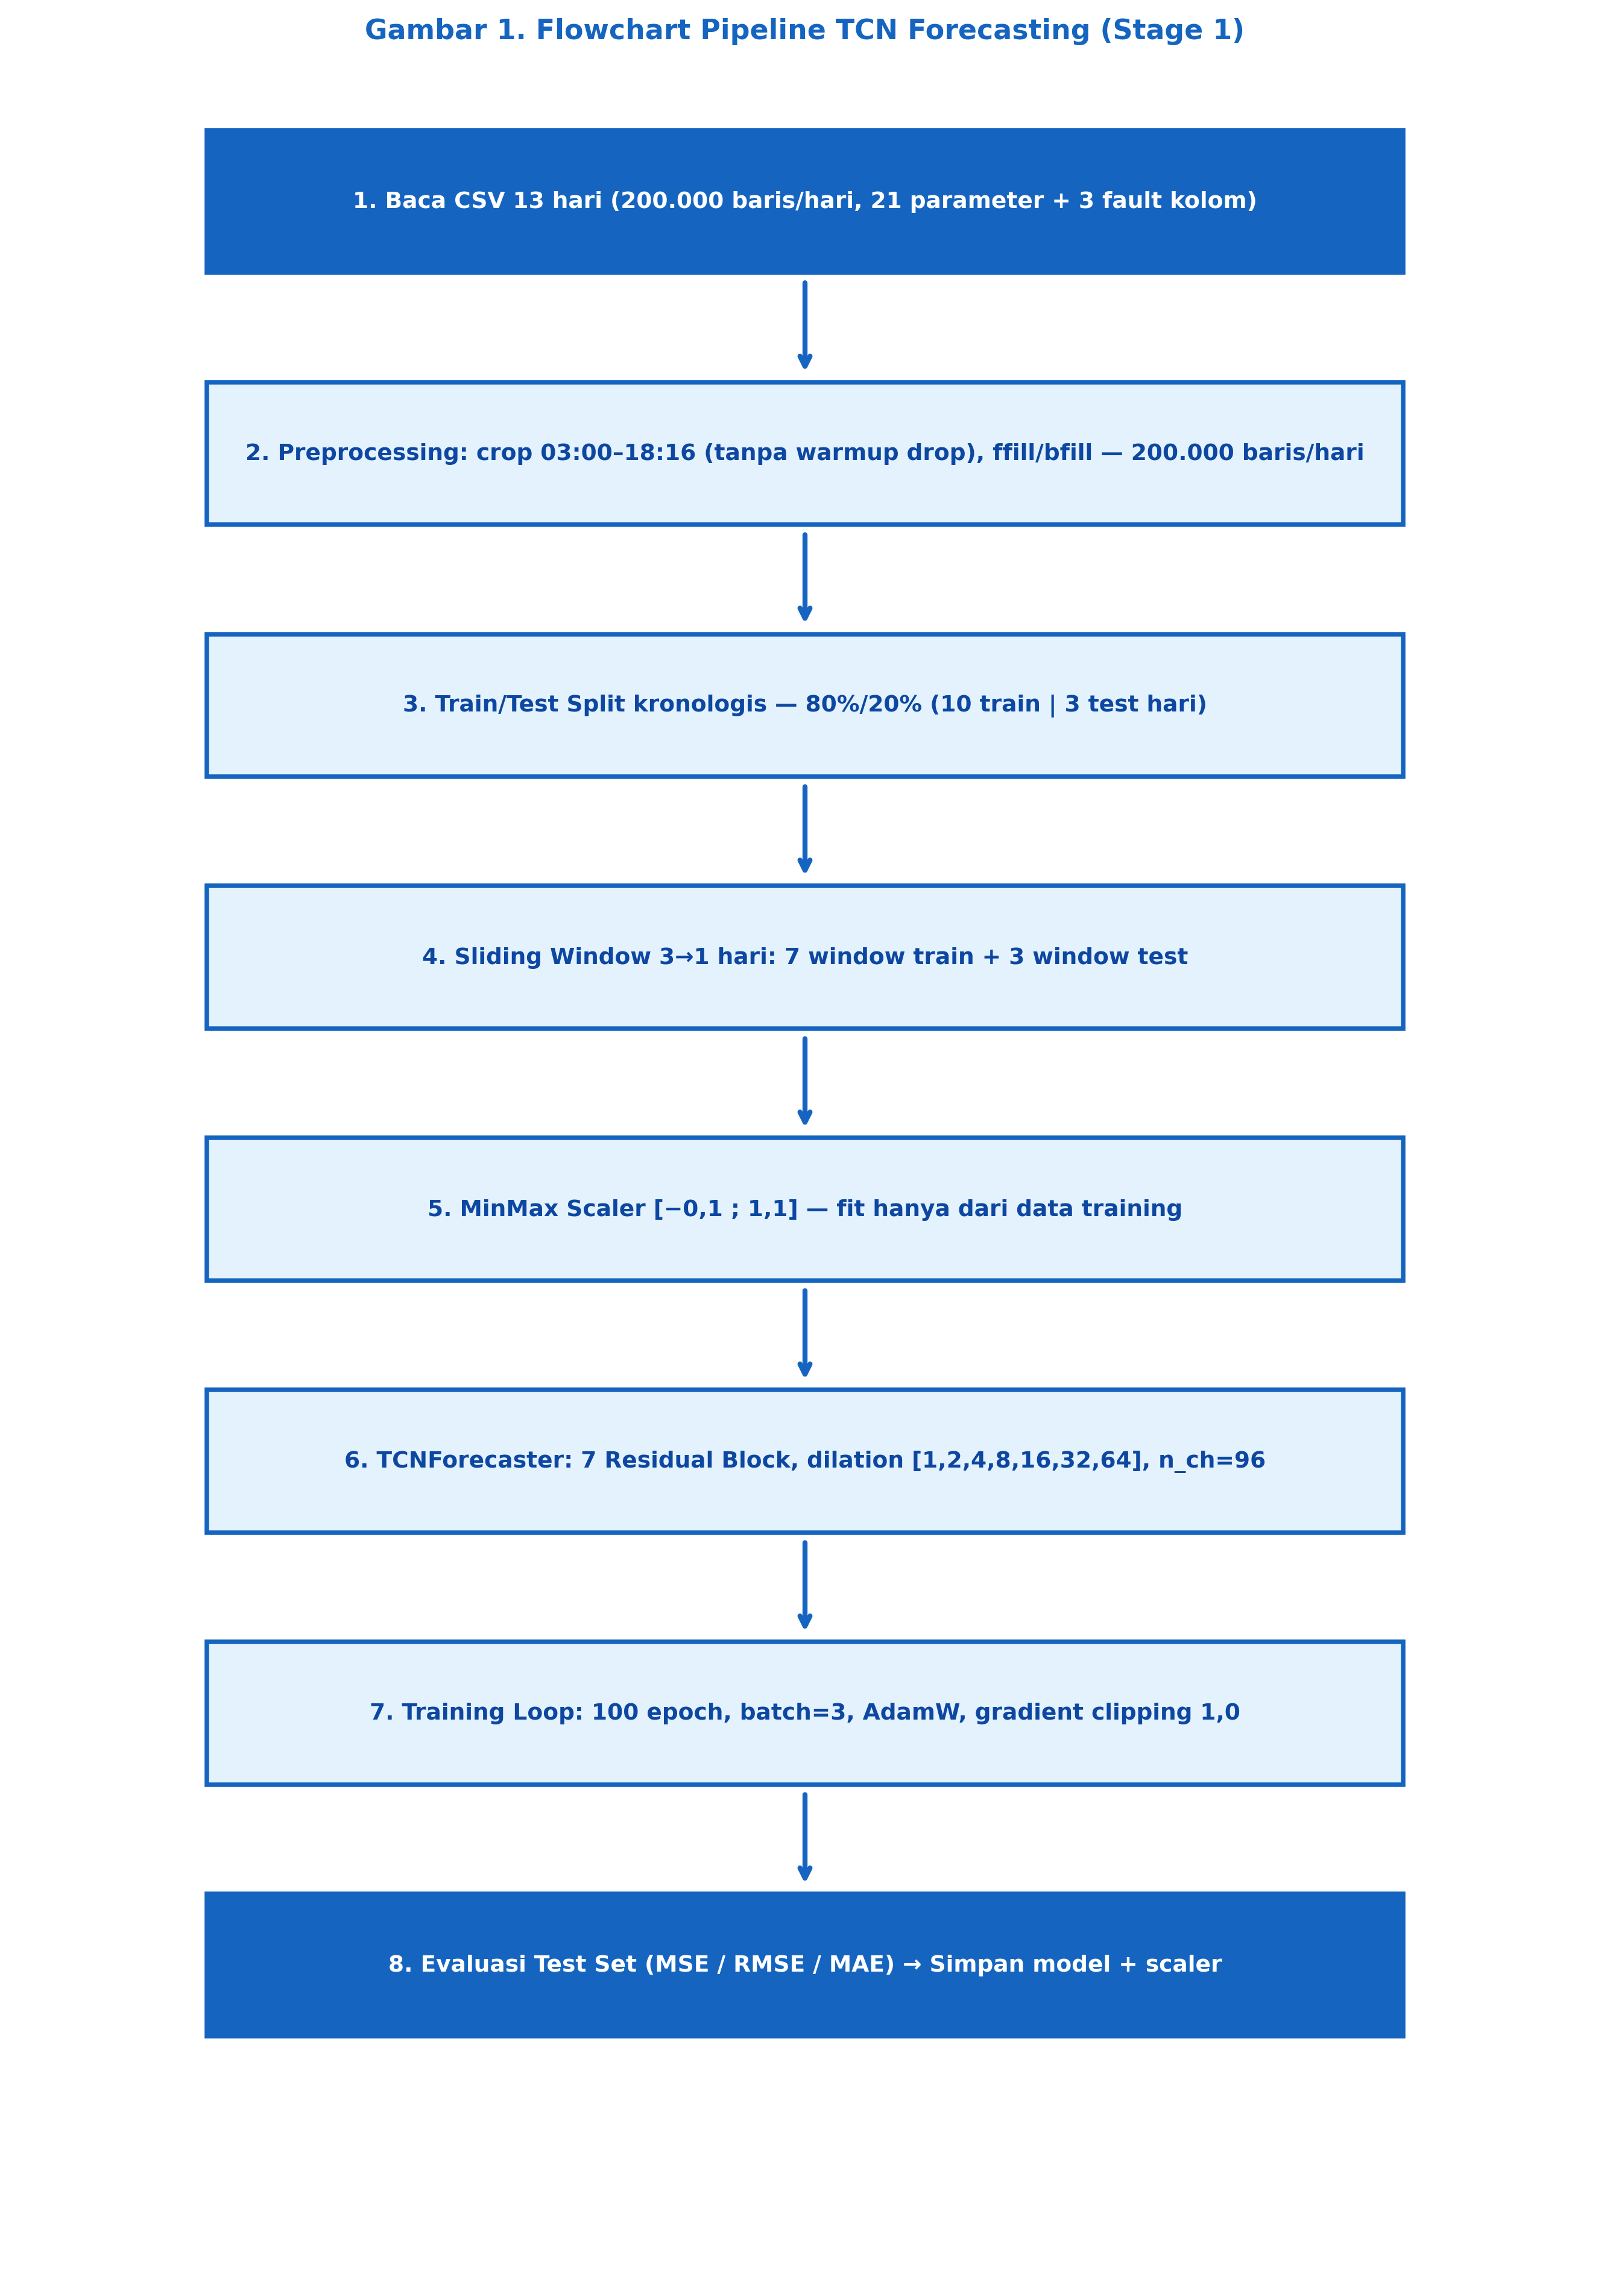
\includegraphics[width=\linewidth]{jurnal_flowchart_stage1.png}
    \caption{Diagram alur pipeline Stage 1 — TCN Forecaster.}
    \label{fig:flow1}
\end{figure}

\begin{figure}[H]
    \centering
    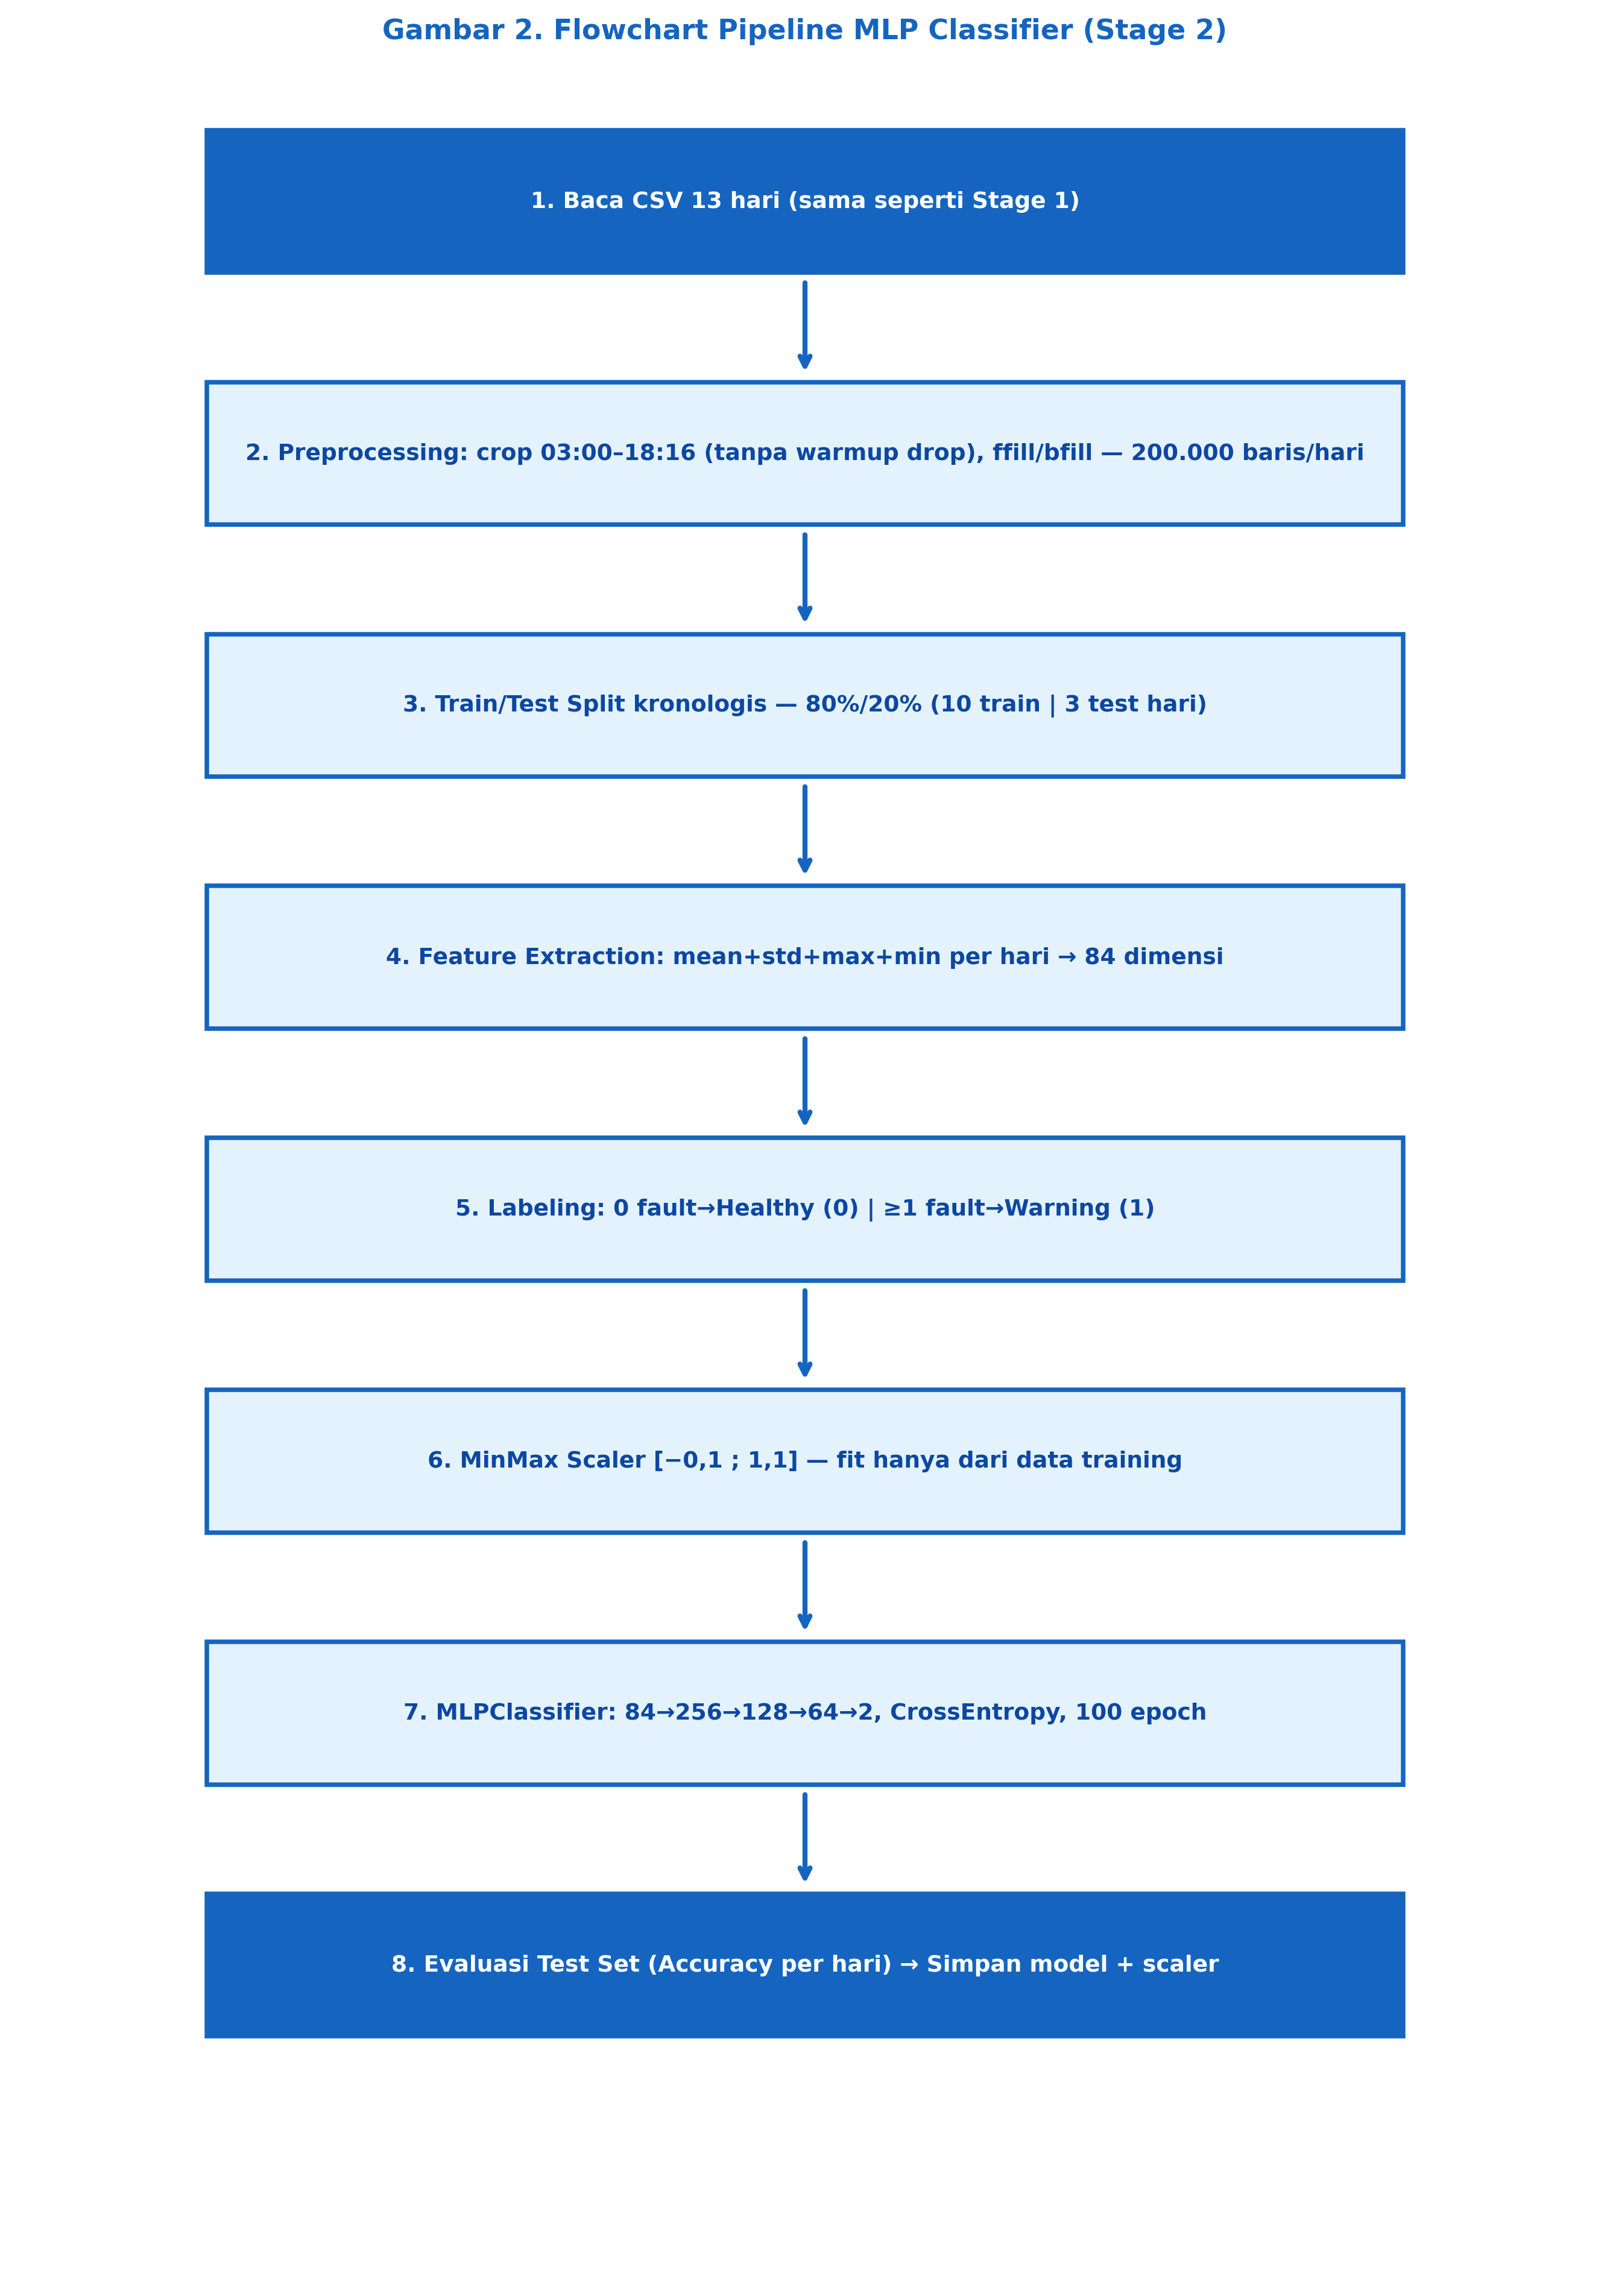
\includegraphics[width=\linewidth]{jurnal_flowchart_stage2.png}
    \caption{Diagram alur pipeline Stage 2 — MLP Classifier.}
    \label{fig:flow2}
\end{figure}

\subsection{Dataset}
Dataset terdiri atas 37 hari data valid unit SIV TS27, masing-masing 200.000 baris (21 parameter), dengan pembagian kronologis 29 hari \textit{training} dan 8 hari \textit{testing} (Tabel~\ref{tab:summary}). \textit{Missing value} ditangani dengan forward-fill dan backward-fill.

\begin{table}[H]
    \centering
    \small
    \caption{Ringkasan dataset SIV TS27.}
    \label{tab:summary}
    \begin{tabular}{ll}
        \toprule
        \textbf{Keterangan} & \textbf{Nilai} \\
        \midrule
        Total hari CSV valid & 37 hari \\
        Hari \textit{training} / \textit{testing} & 29 / 8 hari \\
        Baris per hari & 200.000 \\
        Total baris digunakan & 7.400.000 \\
        Jumlah parameter & 21 \\
        Window \textit{training} / \textit{testing} & 26 / 8 \\
        Distribusi label (37 hari) & 25 \healthy\ / 12 \warning \\
        \bottomrule
    \end{tabular}
\end{table}

\begin{figure}[H]
    \centering
    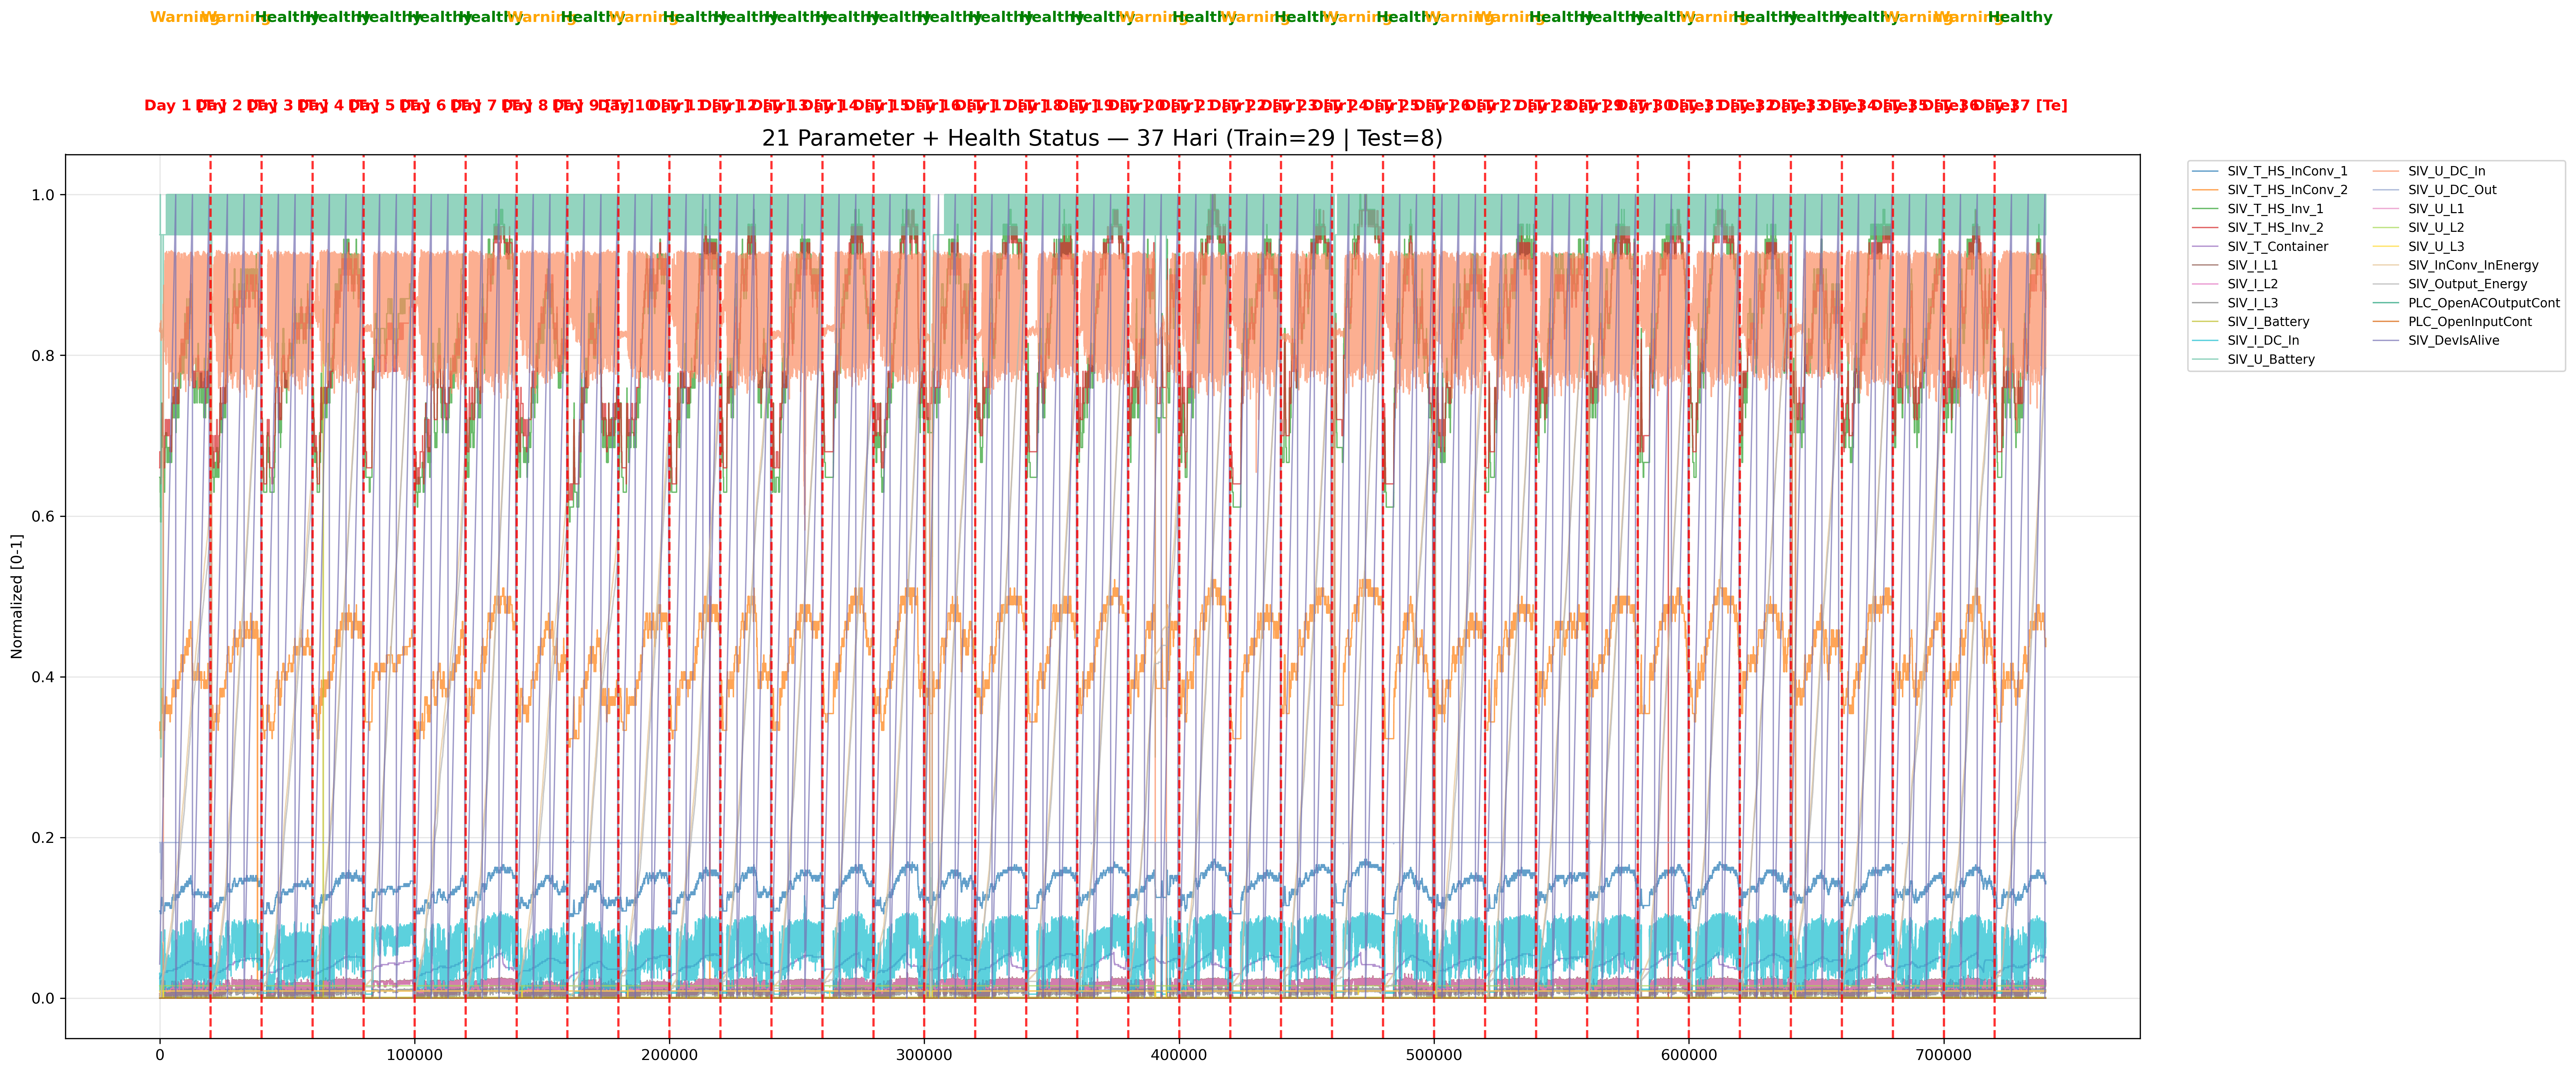
\includegraphics[width=\linewidth]{plot_all_parameters_TCN.png}
    \caption{Plot 21 parameter sensor untuk seluruh hari dataset.}
    \label{fig:allparam}
\end{figure}

\subsection{Normalisasi dan Sliding Window}
Seluruh parameter dinormalisasi dengan \textbf{Min-Max Scaler} ke rentang $[-0,1;\ 1,1]$, di-\textit{fit} hanya pada data \textit{training} untuk mencegah kebocoran data. Sequence input-output dibentuk dengan skema \textit{sliding window} 3 hari input $\to$ 1 hari target, digeser satu hari setiap langkah (Gambar~\ref{fig:norm} dan~\ref{fig:slidewin}).

\begin{figure}[H]
    \centering
    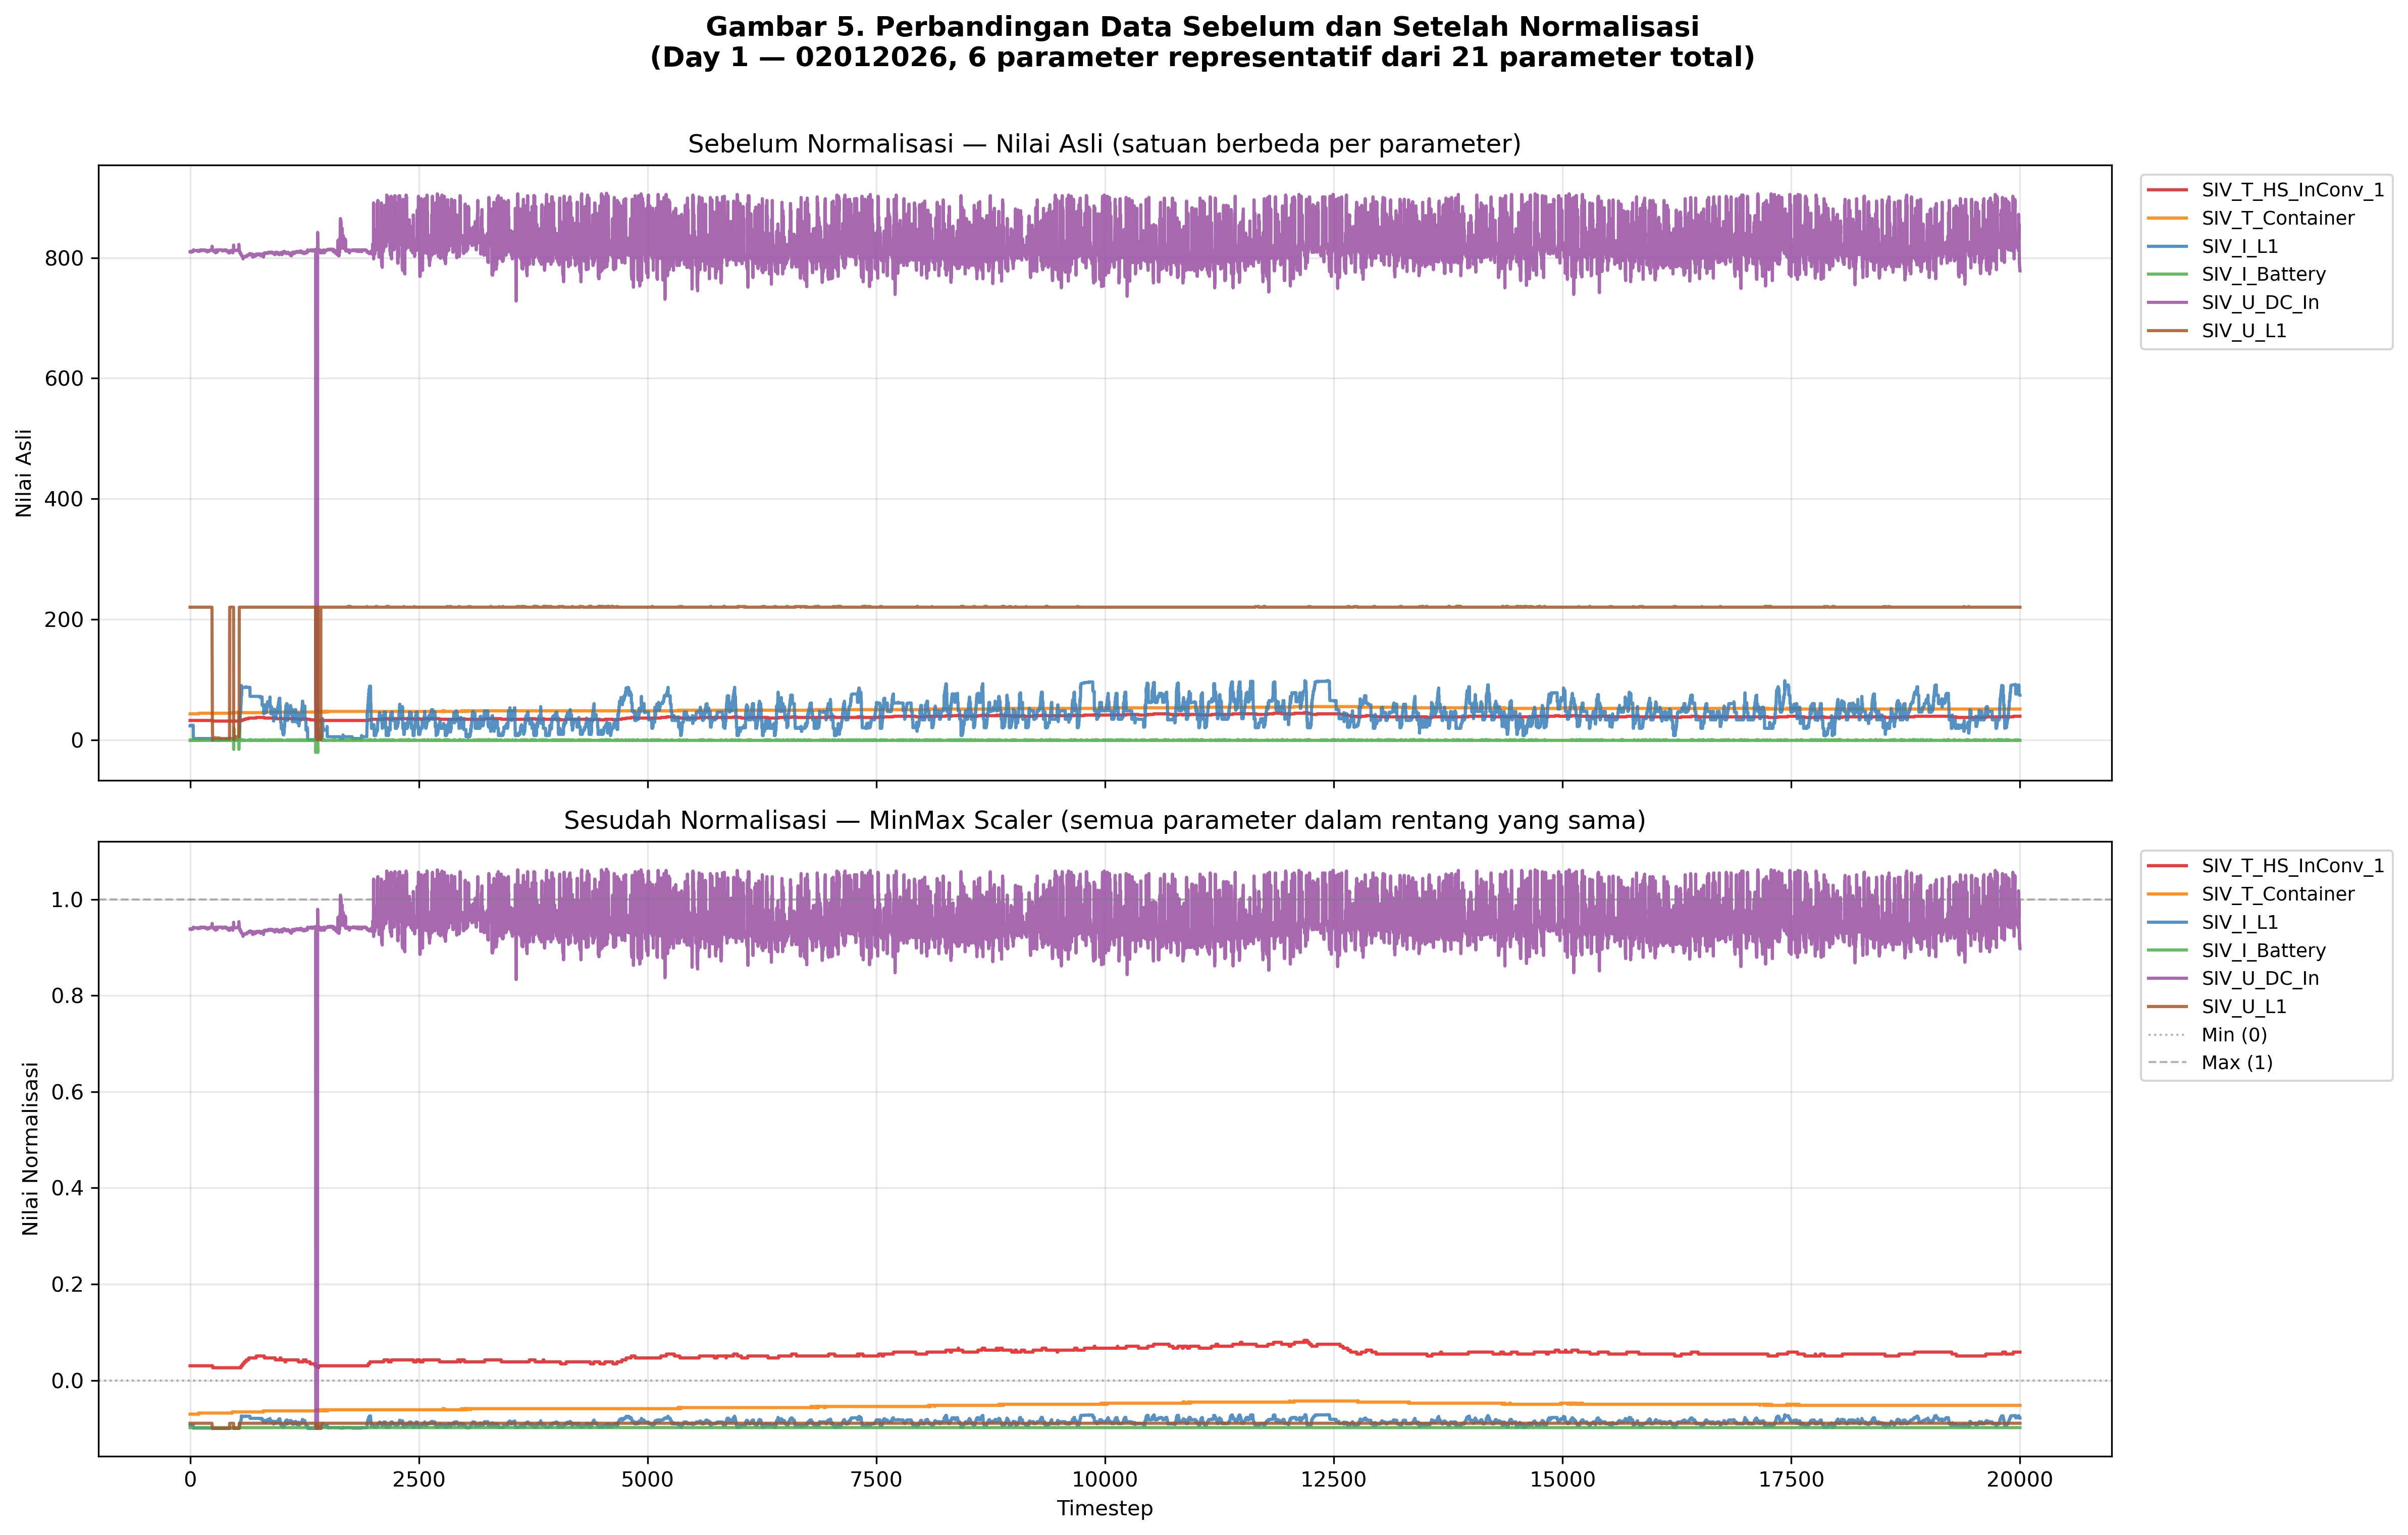
\includegraphics[width=0.9\linewidth]{jurnal_normalisasi_comparison.png}
    \caption{Perbandingan data sebelum vs sesudah normalisasi Min-Max.}
    \label{fig:norm}
\end{figure}

\begin{figure}[H]
    \centering
    \includegraphics[width=0.8\linewidth]{jurnal_sliding_window.png}
    \caption{Skema sliding window: 3 hari input memprediksi 1 hari target berikutnya.}
    \label{fig:slidewin}
\end{figure}

\subsection{Arsitektur dan Hyperparameter}
\begin{table}[H]
    \centering
    \small
    \caption{Arsitektur dan hyperparameter Stage 1 (TCN).}
    \begin{tabular}{ll}
        \toprule
        \textbf{Parameter} & \textbf{Nilai} \\
        \midrule
        Residual Block & 7 \\
        Dilation Factors & 1,2,4,8,16,32,64 \\
        Hidden Channel & 96 \\
        Kernel Size & 3 \\
        Input / Output & 3 hari / 1 hari \\
        Optimizer & AdamW (LR 0,001) \\
        Batch Size / Epoch & 3 / 100 \\
        Loss & MSE \\
        Dropout / Weight Decay & 0,3 / 1e-5 \\
        \bottomrule
    \end{tabular}
    \hspace{0.5cm}
    \caption{Arsitektur dan hyperparameter Stage 2 (MLP).}
    \begin{tabular}{ll}
        \toprule
        \textbf{Parameter} & \textbf{Nilai} \\
        \midrule
        Input & 84 fitur statistik \\
        Hidden Layers & 256-128-64 (LayerNorm+ReLU) \\
        Output & 2 (Softmax) \\
        Optimizer & AdamW (LR 0,001) \\
        Batch Size / Epoch & 3 / 100 \\
        Loss & Cross-Entropy \\
        Class Weight & Healthy=0,5, Warning=2,5 \\
        Dropout / Weight Decay & 0,3 / 1e-5 \\
        \bottomrule
    \end{tabular}
\end{table}

% ============================================================
\section{Hasil dan Pembahasan}
% ============================================================

\subsection{Hasil Training Stage 1 — TCN Forecaster}
MSE menurun dari 0,3568 (epoch 1) menjadi 0,0120 (epoch 100), penurunan 96,6\% (Gambar~\ref{fig:loss1}).

\begin{figure}[H]
    \centering
    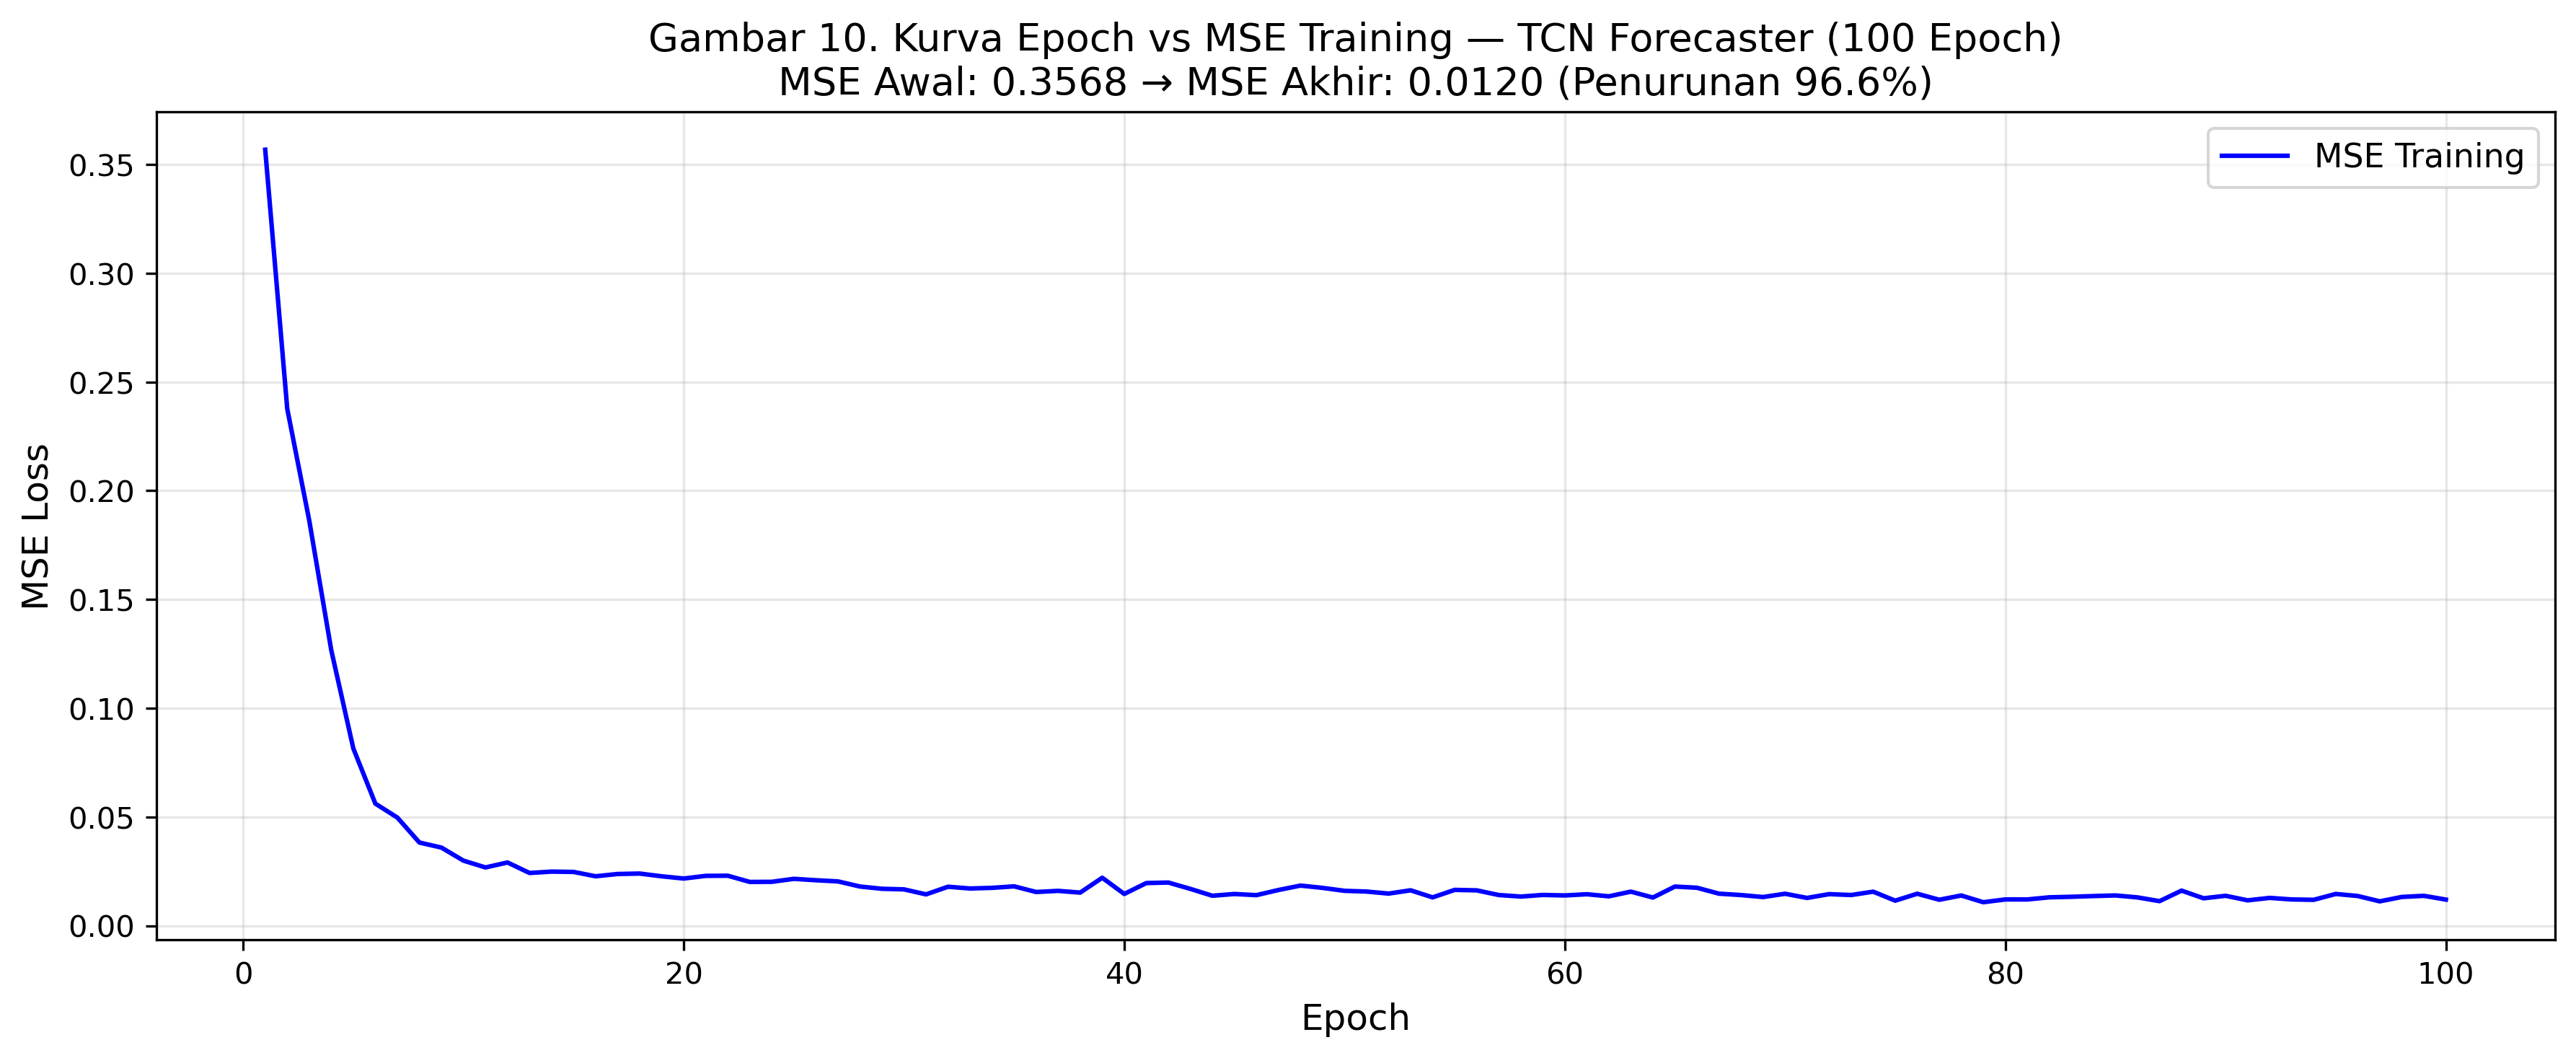
\includegraphics[width=0.85\linewidth]{jurnal_kurva_loss_stage1.png}
    \caption{Kurva Epoch vs MSE Stage 1 (TCN Forecaster).}
    \label{fig:loss1}
\end{figure}

\begin{table}[H]
    \centering
    \caption{Evaluasi Stage 1 pada skala ternormalisasi $[-0,1;\ 1,1]$.}
    \begin{tabular}{lrr}
        \toprule
        \textbf{Metrik} & \textbf{Training} & \textbf{Testing} \\
        \midrule
        MSE  & 0,008066 & 0,007446 \\
        RMSE & 0,089810 & 0,086292 \\
        MAE  & 0,046303 & 0,043340 \\
        MAPE & 44,83\%  & 42,43\% \\
        \bottomrule
    \end{tabular}
\end{table}

\noindent Selisih MSE \textit{train--test} kecil (0,00456), menunjukkan model TCN \textbf{tidak overfitting} dan generalisasi dengan baik.

\subsection{Hasil Training Stage 2 — MLP Classifier}
CE Loss menurun dari 1,0051 menjadi 0,0682 (93,2\%); akurasi \textit{training} meningkat dari 66,67\% menjadi 96,30--100\% (Gambar~\ref{fig:loss2}).

\begin{figure}[H]
    \centering
    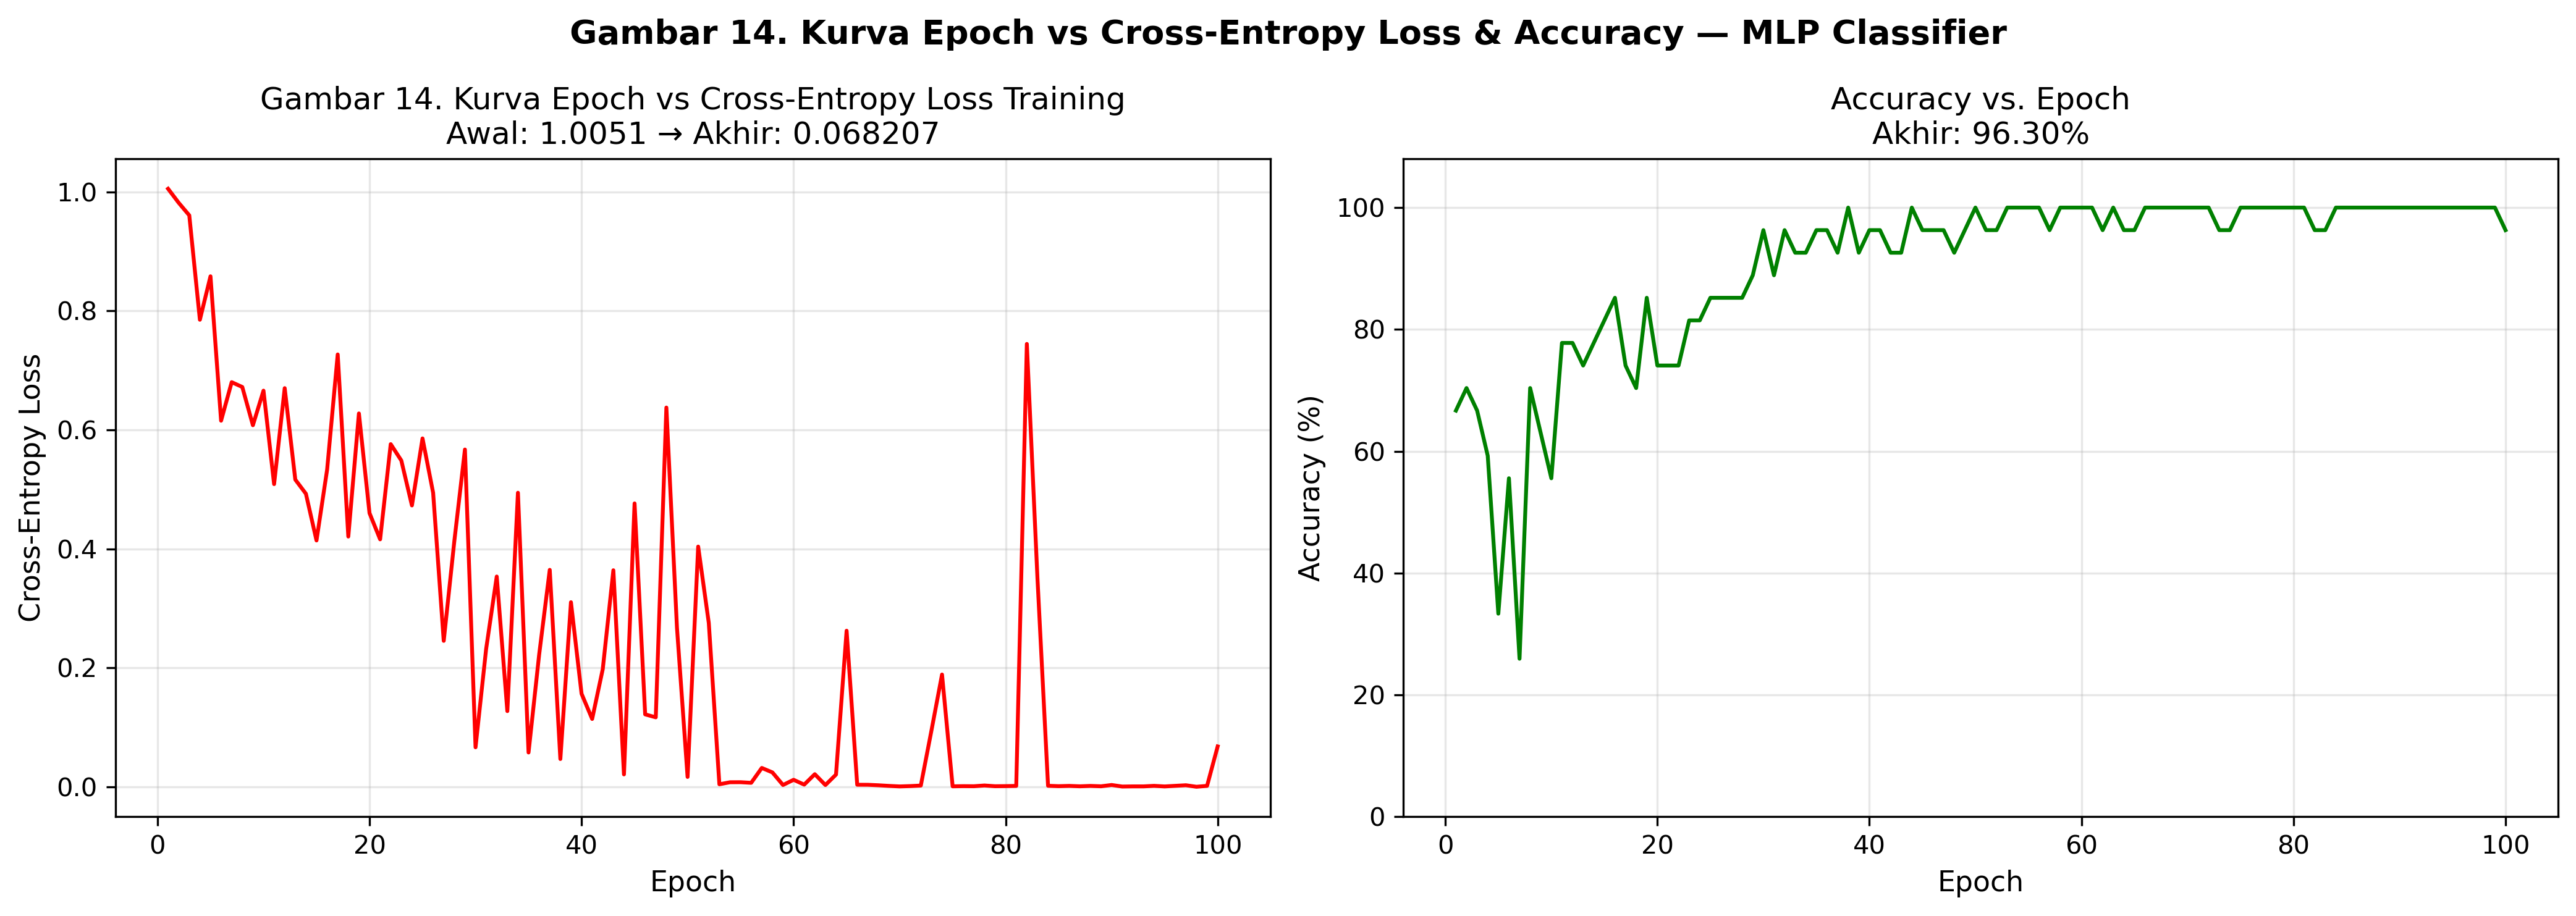
\includegraphics[width=0.85\linewidth]{jurnal_kurva_loss_acc_stage2.png}
    \caption{Kurva CE Loss dan Accuracy Stage 2 (MLP Classifier).}
    \label{fig:loss2}
\end{figure}

\begin{table}[H]
    \centering
    \caption{Evaluasi Stage 2 — Training vs Testing.}
    \begin{tabular}{lrr}
        \toprule
        \textbf{Metrik} & \textbf{Training} & \textbf{Testing} \\
        \midrule
        CE Loss   & 0,000223 & 5,903700 \\
        Accuracy  & 100,00\% & 62,50\% \\
        Precision & 100,00\% & 39,06\% \\
        Recall    & 100,00\% & 62,50\% \\
        F1-Score  & 100,00\% & 48,08\% \\
        \bottomrule
    \end{tabular}
\end{table}

\begin{figure}[H]
    \centering
    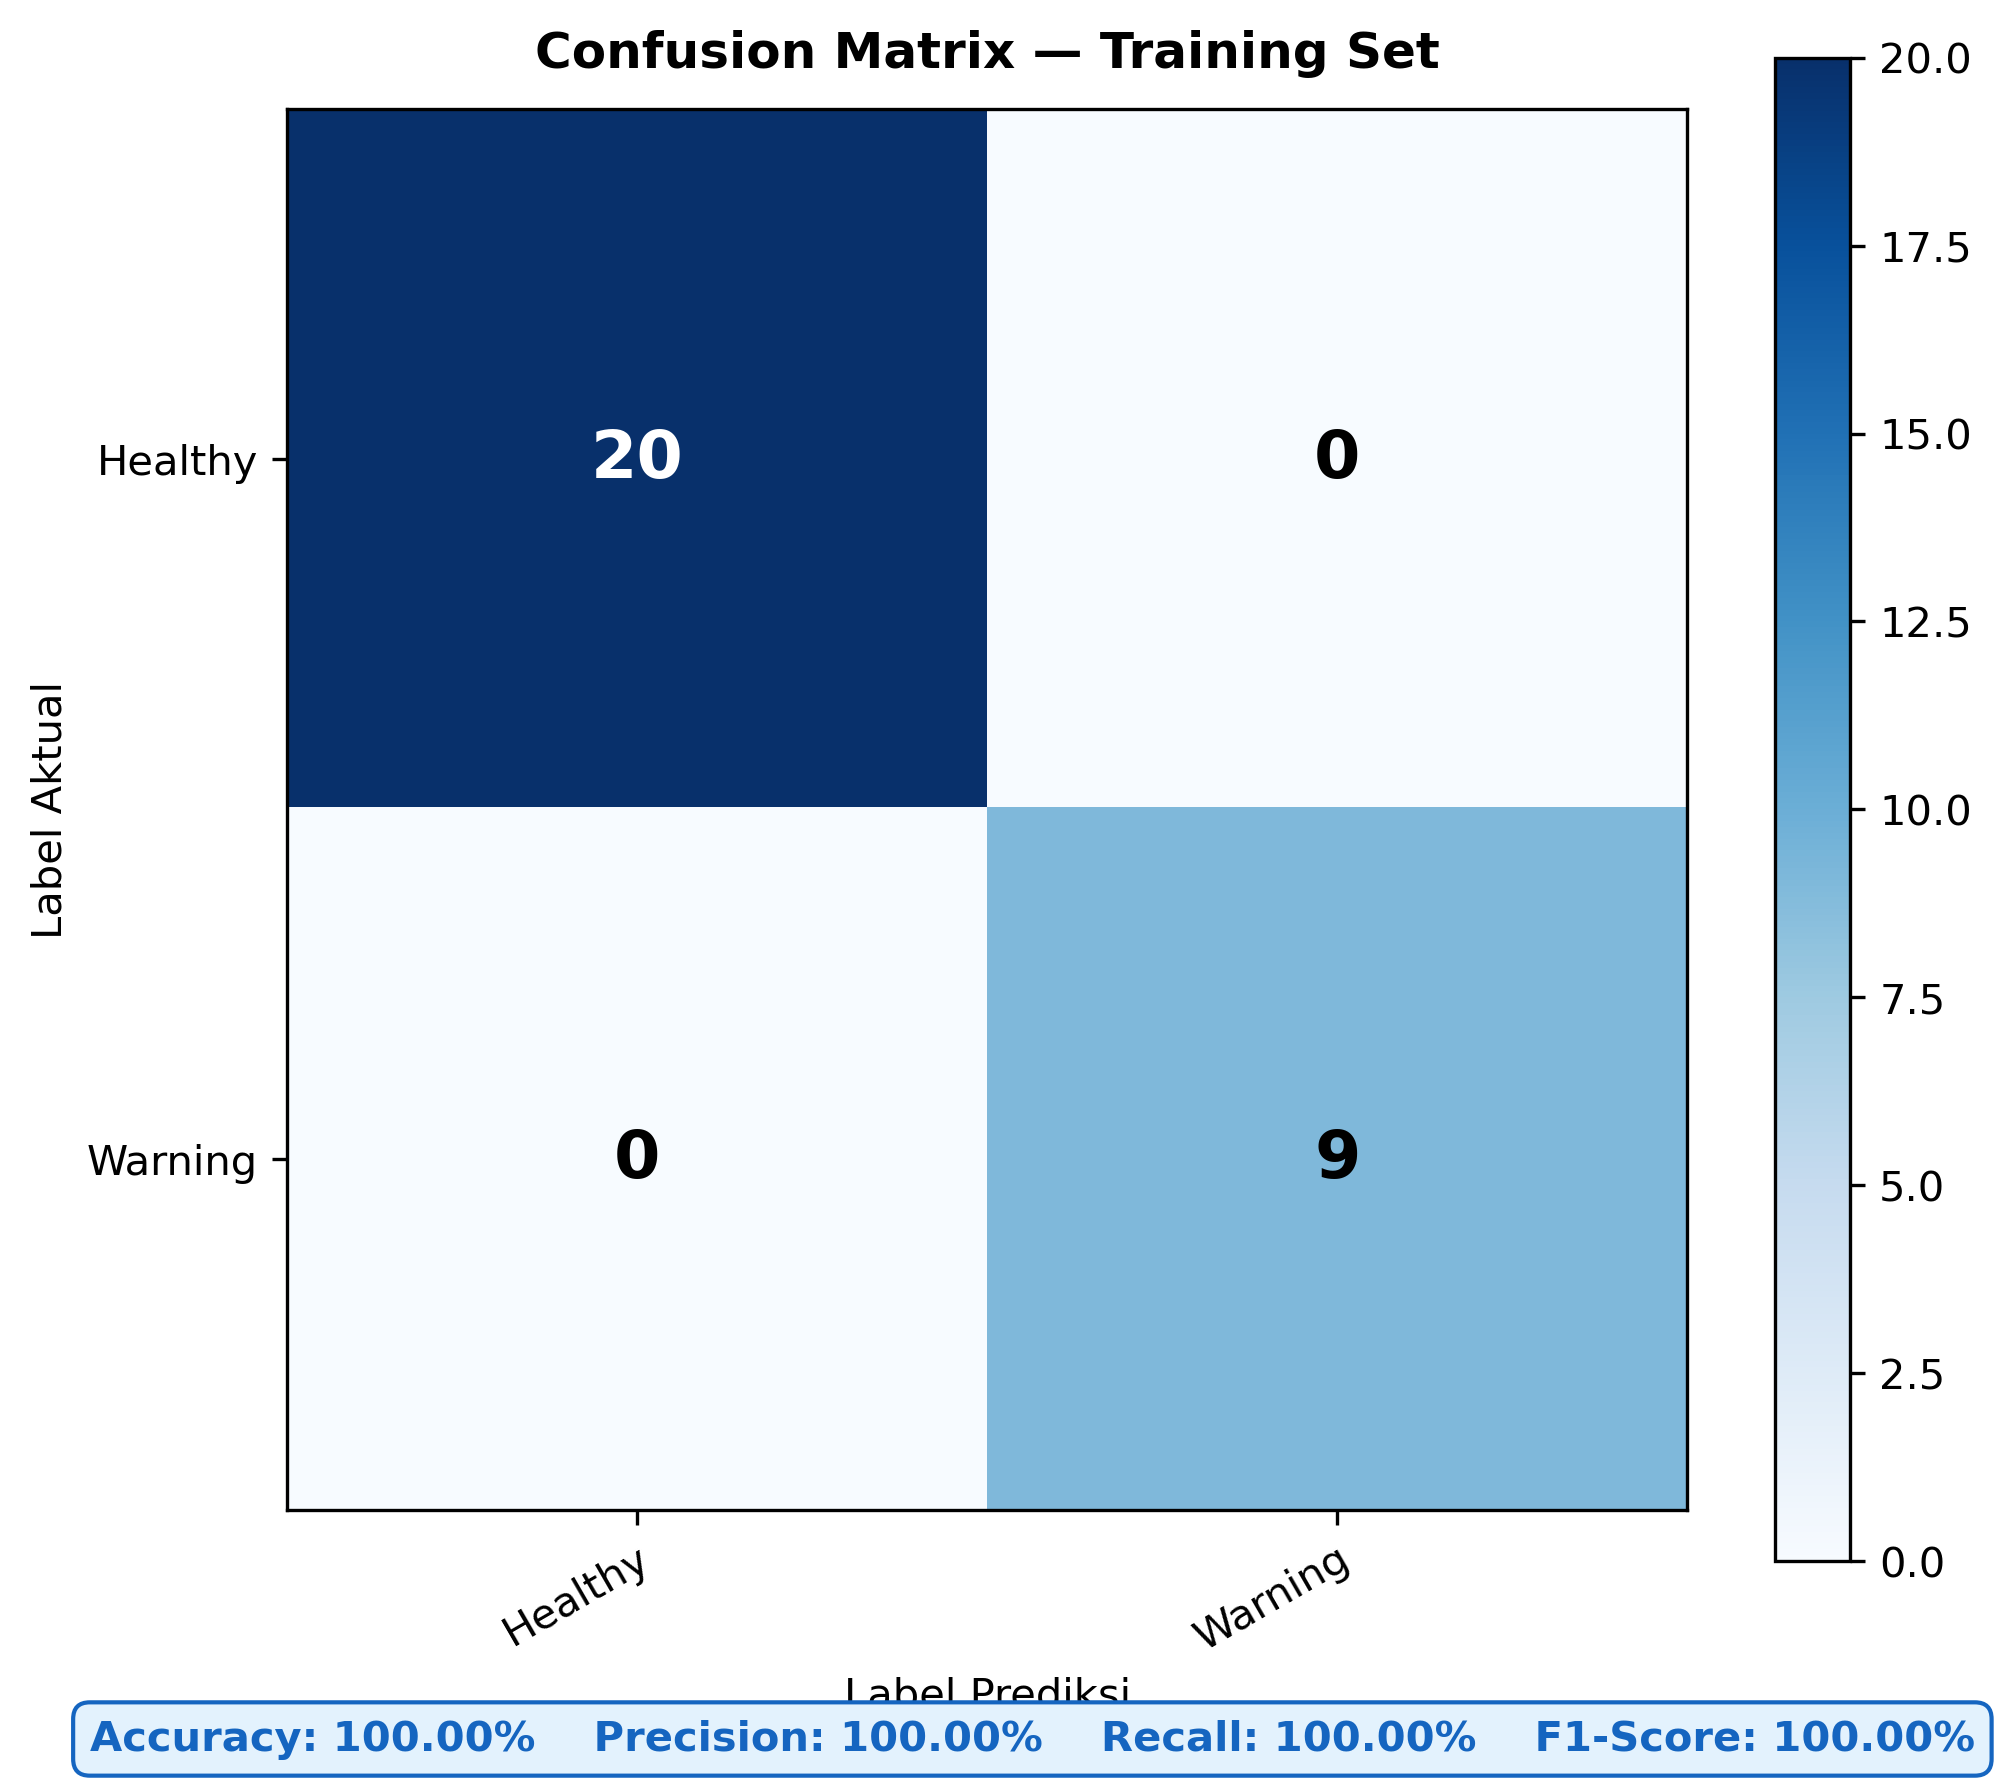
\includegraphics[width=0.75\linewidth]{jurnal_confusion_matrix_train.png}
    \caption{Confusion matrix Training — Acc/Prec/Rec/F1 = 100,00\%.}
    \label{fig:cmtrain}
\end{figure}

\begin{figure}[H]
    \centering
    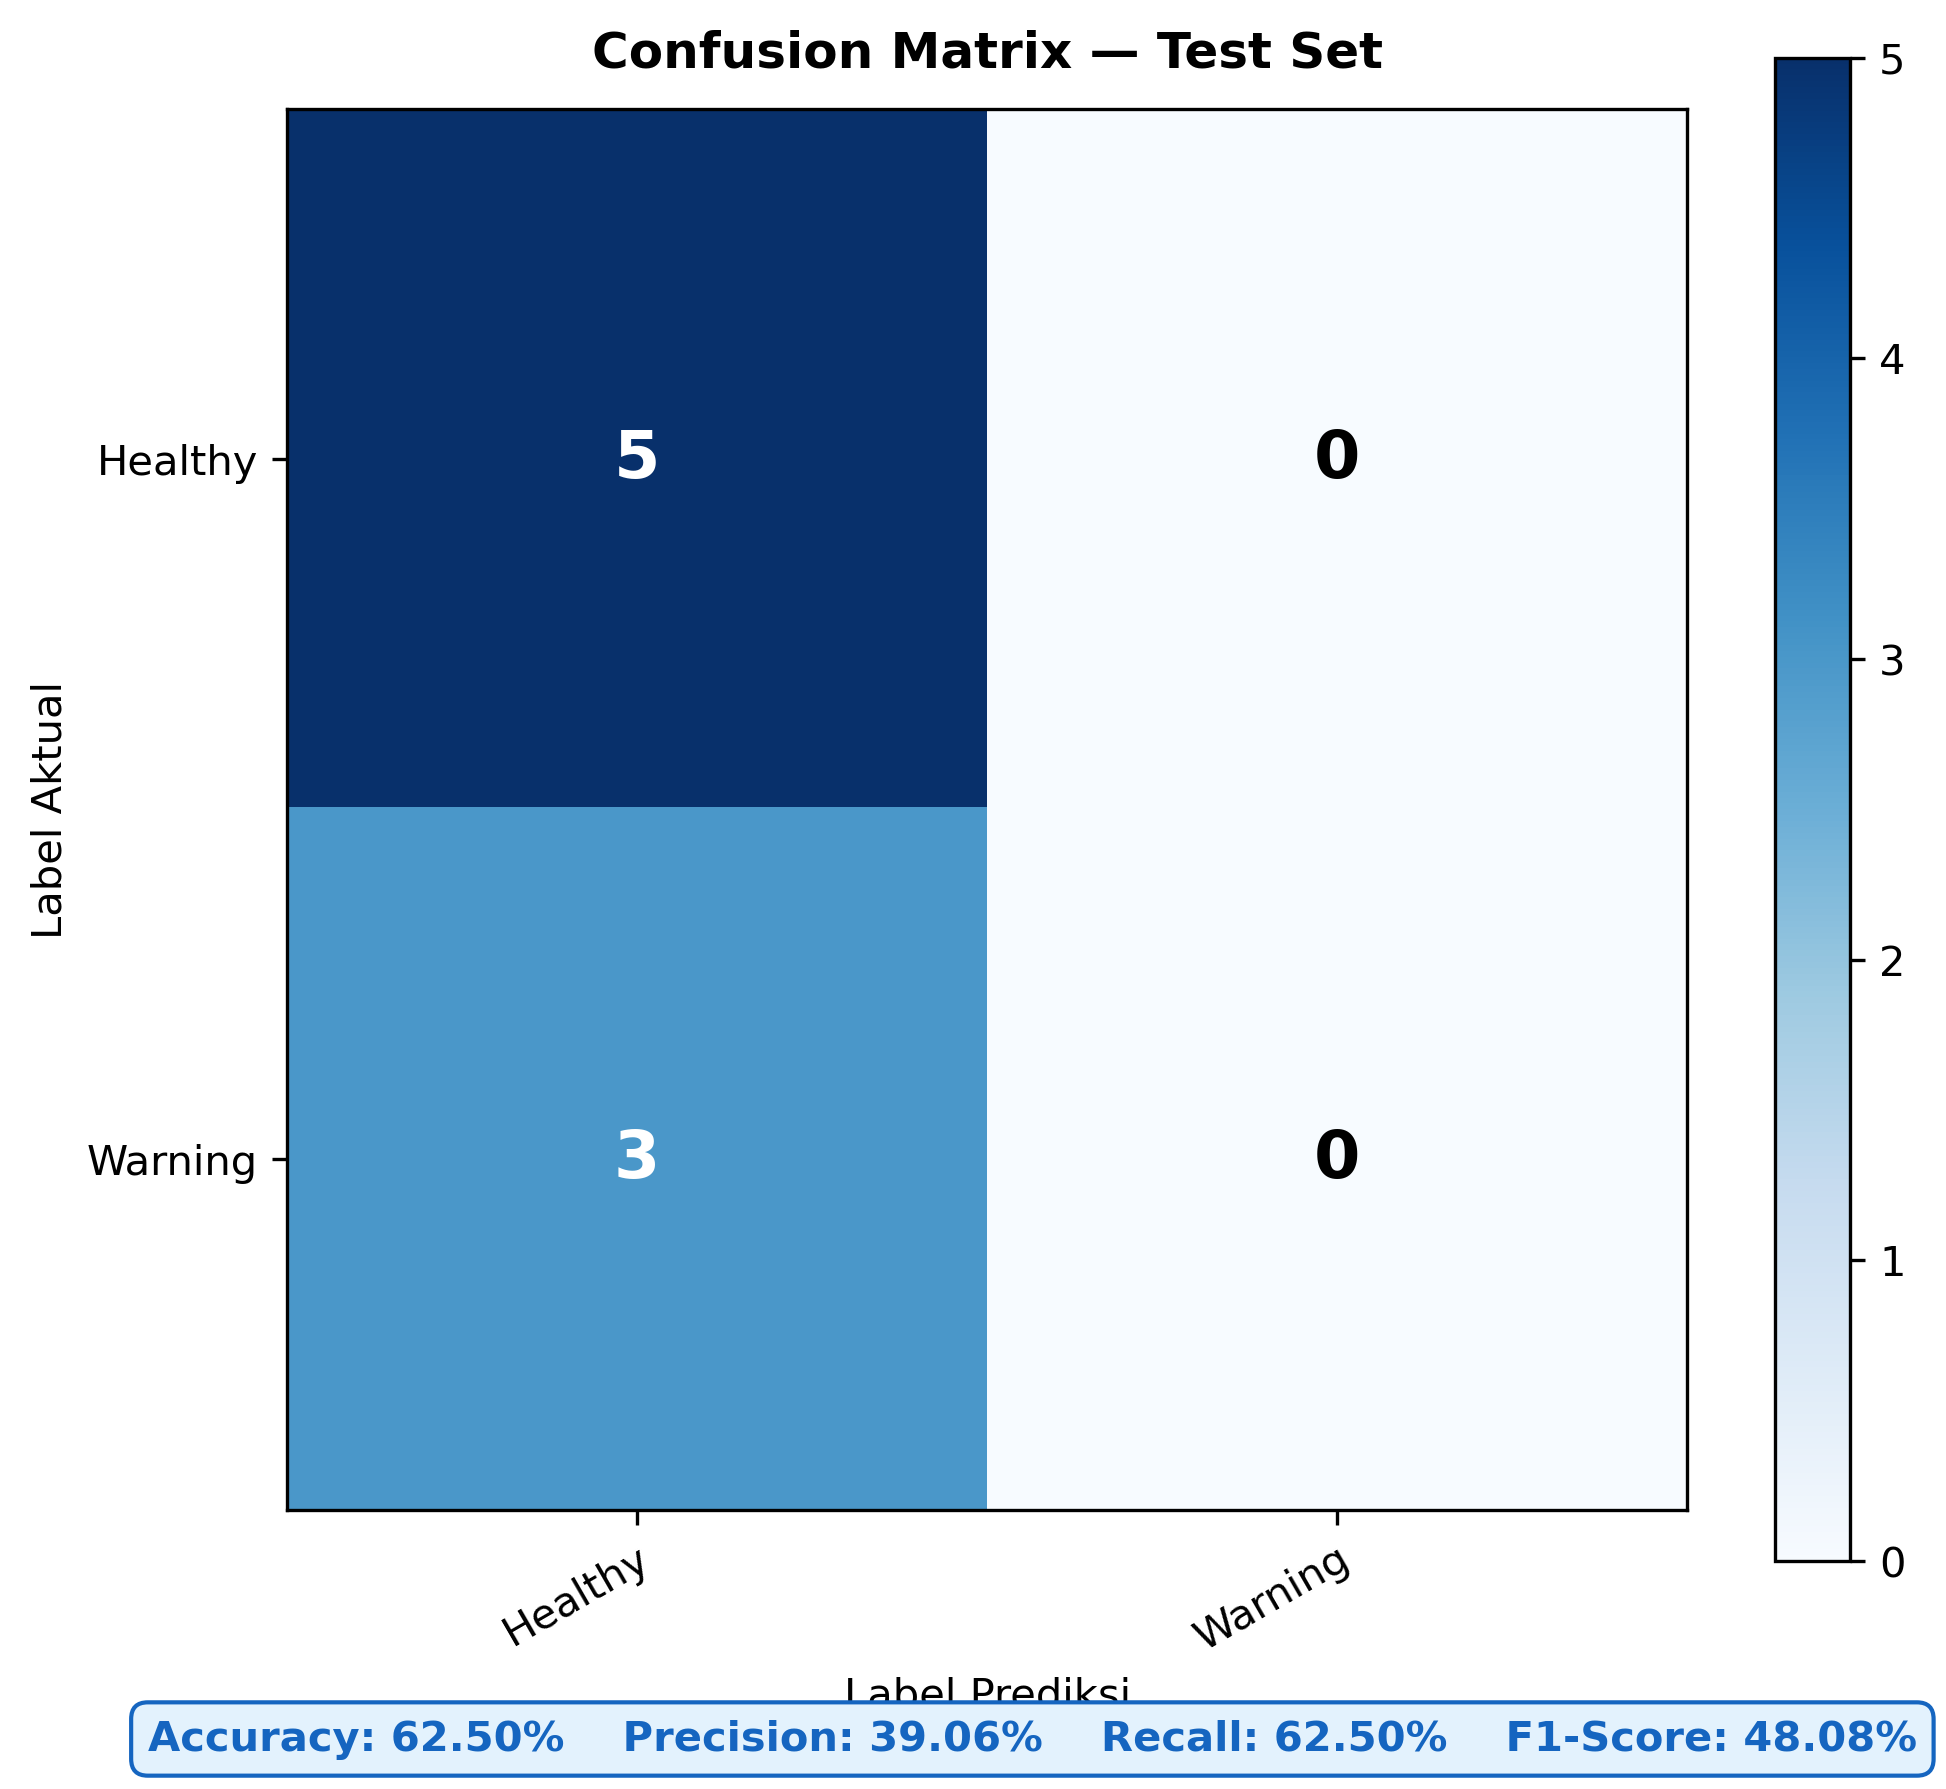
\includegraphics[width=0.75\linewidth]{jurnal_confusion_matrix_test.png}
    \caption{Confusion matrix Testing — Acc=62,50\%, Prec=39,06\%, Rec=62,50\%, F1=48,08\%.}
    \label{fig:cmtest}
\end{figure}

\begin{table}[H]
    \centering
    \small
    \caption{Detail prediksi per hari — Test Set.}
    \begin{tabular}{clllc}
        \toprule
        \textbf{Day} & \textbf{Tanggal} & \textbf{Aktual} & \textbf{Prediksi} & \textbf{Benar?} \\
        \midrule
        30 & 09052026 & \healthy & \healthy & \ok \\
        31 & 14052026 & \warning & \healthy & \bad \\
        32 & 15052026 & \healthy & \healthy & \ok \\
        33 & 16052026 & \healthy & \healthy & \ok \\
        34 & 17052026 & \healthy & \healthy & \ok \\
        35 & 20052026 & \warning & \healthy & \bad \\
        36 & 22052026 & \warning & \healthy & \bad \\
        37 & 23052026 & \healthy & \healthy & \ok \\
        \bottomrule
    \end{tabular}
\end{table}

\begin{figure}[H]
    \centering
    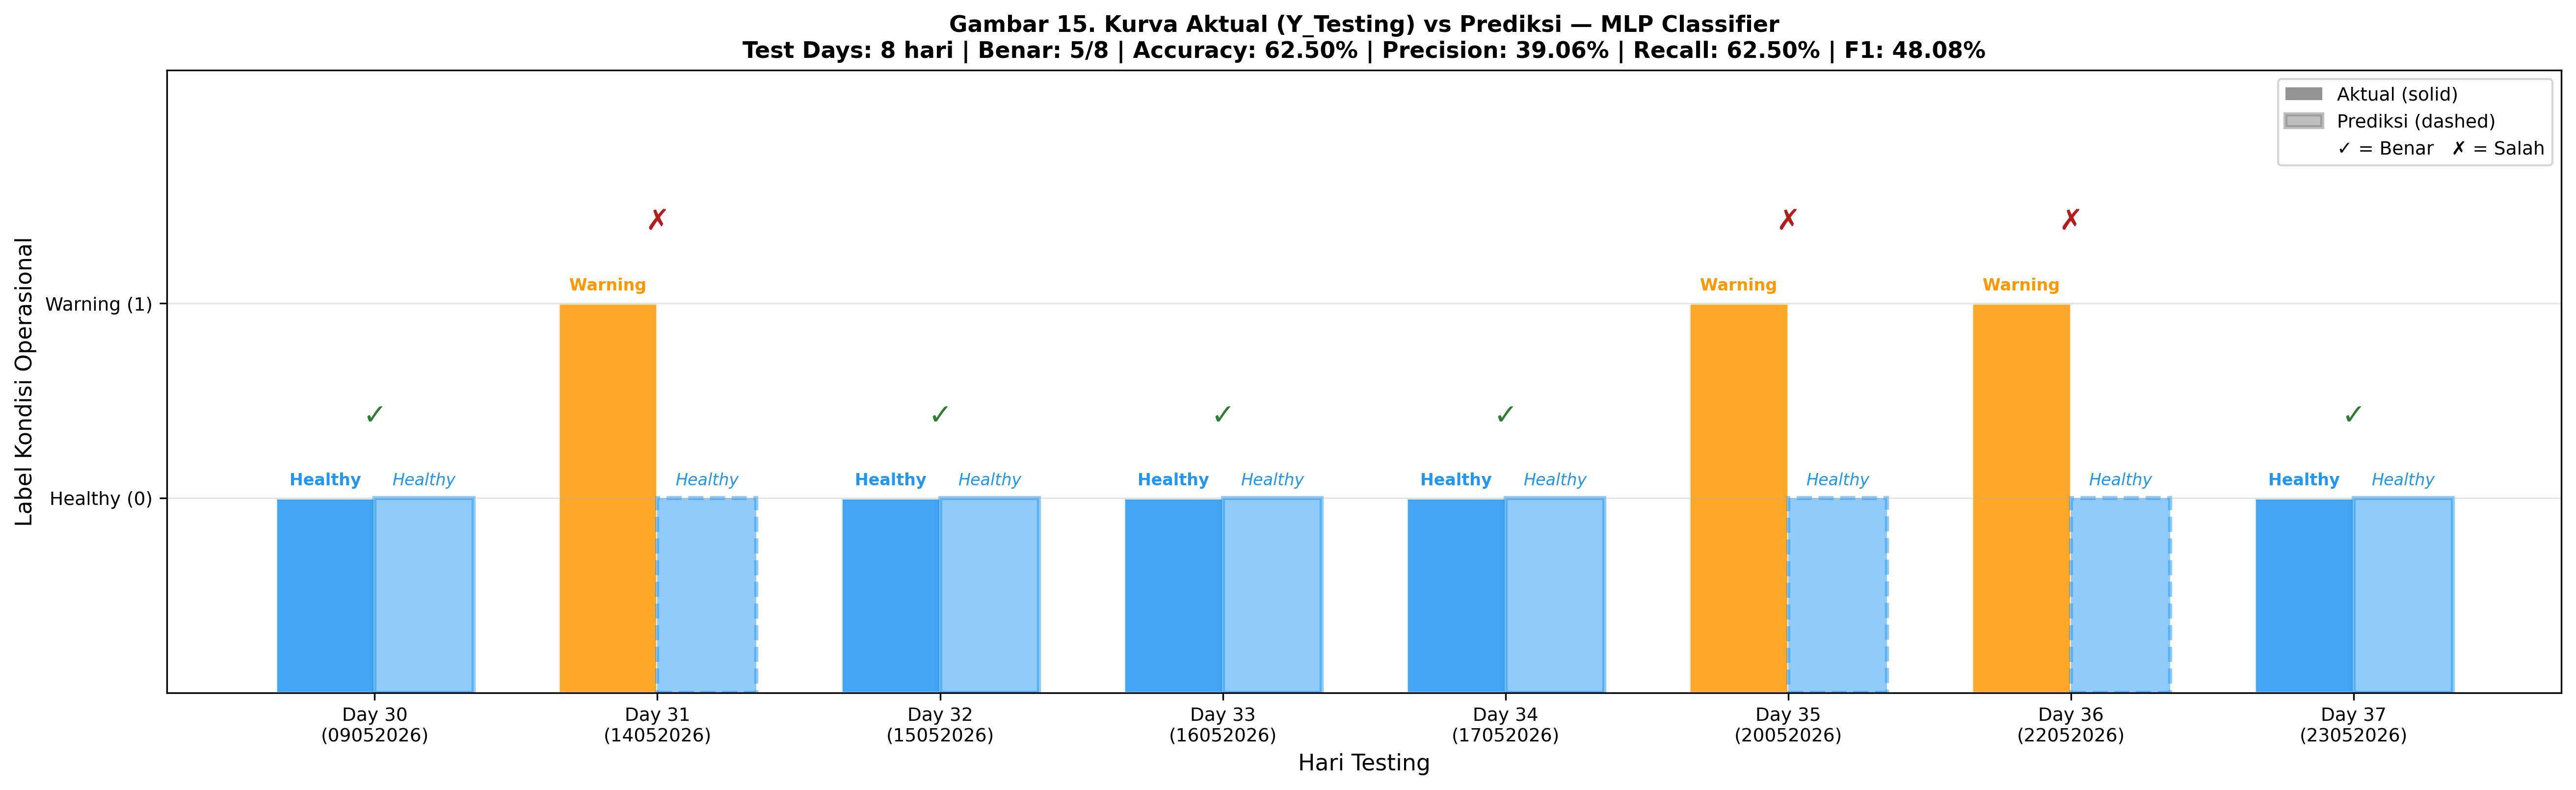
\includegraphics[width=0.85\linewidth]{jurnal_aktual_vs_prediksi_mlp.png}
    \caption{Perbandingan status aktual vs prediksi MLP Classifier per hari.}
    \label{fig:aktualpred}
\end{figure}

\noindent \textbf{Analisis overfitting:} model memprediksi \healthy\ untuk seluruh 8 hari \textit{test}, sehingga ketiga hari \warning\ aktual (Day 31, 35, 36) seluruhnya salah diklasifikasikan (\textit{recall} Warning = 0\%). Penyebab utama: ukuran dataset klasifikasi sangat kecil (29 sampel, 9 di antaranya Warning), tidak ada \textit{early stopping}, dan model bias ke kelas mayoritas.

\subsection{Inference}
Dua skenario inference dievaluasi: \textbf{Training Inference} (Day 27--29 $\to$ Day 30, ada \textit{ground truth}) dan \textbf{Testing Inference} (Day 35--37 $\to$ Day 38 masa depan, tanpa \textit{ground truth}).

\begin{table}[H]
    \centering
    \small
    \caption{Perbandingan Training Inference vs Testing Inference.}
    \begin{tabular}{lll}
        \toprule
        \textbf{Aspek} & \textbf{Training Inference} & \textbf{Testing Inference} \\
        \midrule
        Input Days & Day 27--29 & Day 35--37 \\
        Target & Day 30 & Day 38 (masa depan) \\
        Prediksi & \healthy\ (100,0\%) & \healthy\ (100,0\%) \\
        Ground Truth & \healthy & Tidak ada \\
        Klasifikasi & \ok\ BENAR & Tdk dpt diukur \\
        MSE/RMSE/MAE & 0,004950/0,070358/0,037082 & Tdk dpt diukur \\
        \bottomrule
    \end{tabular}
\end{table}

\begin{figure}[H]
    \centering
    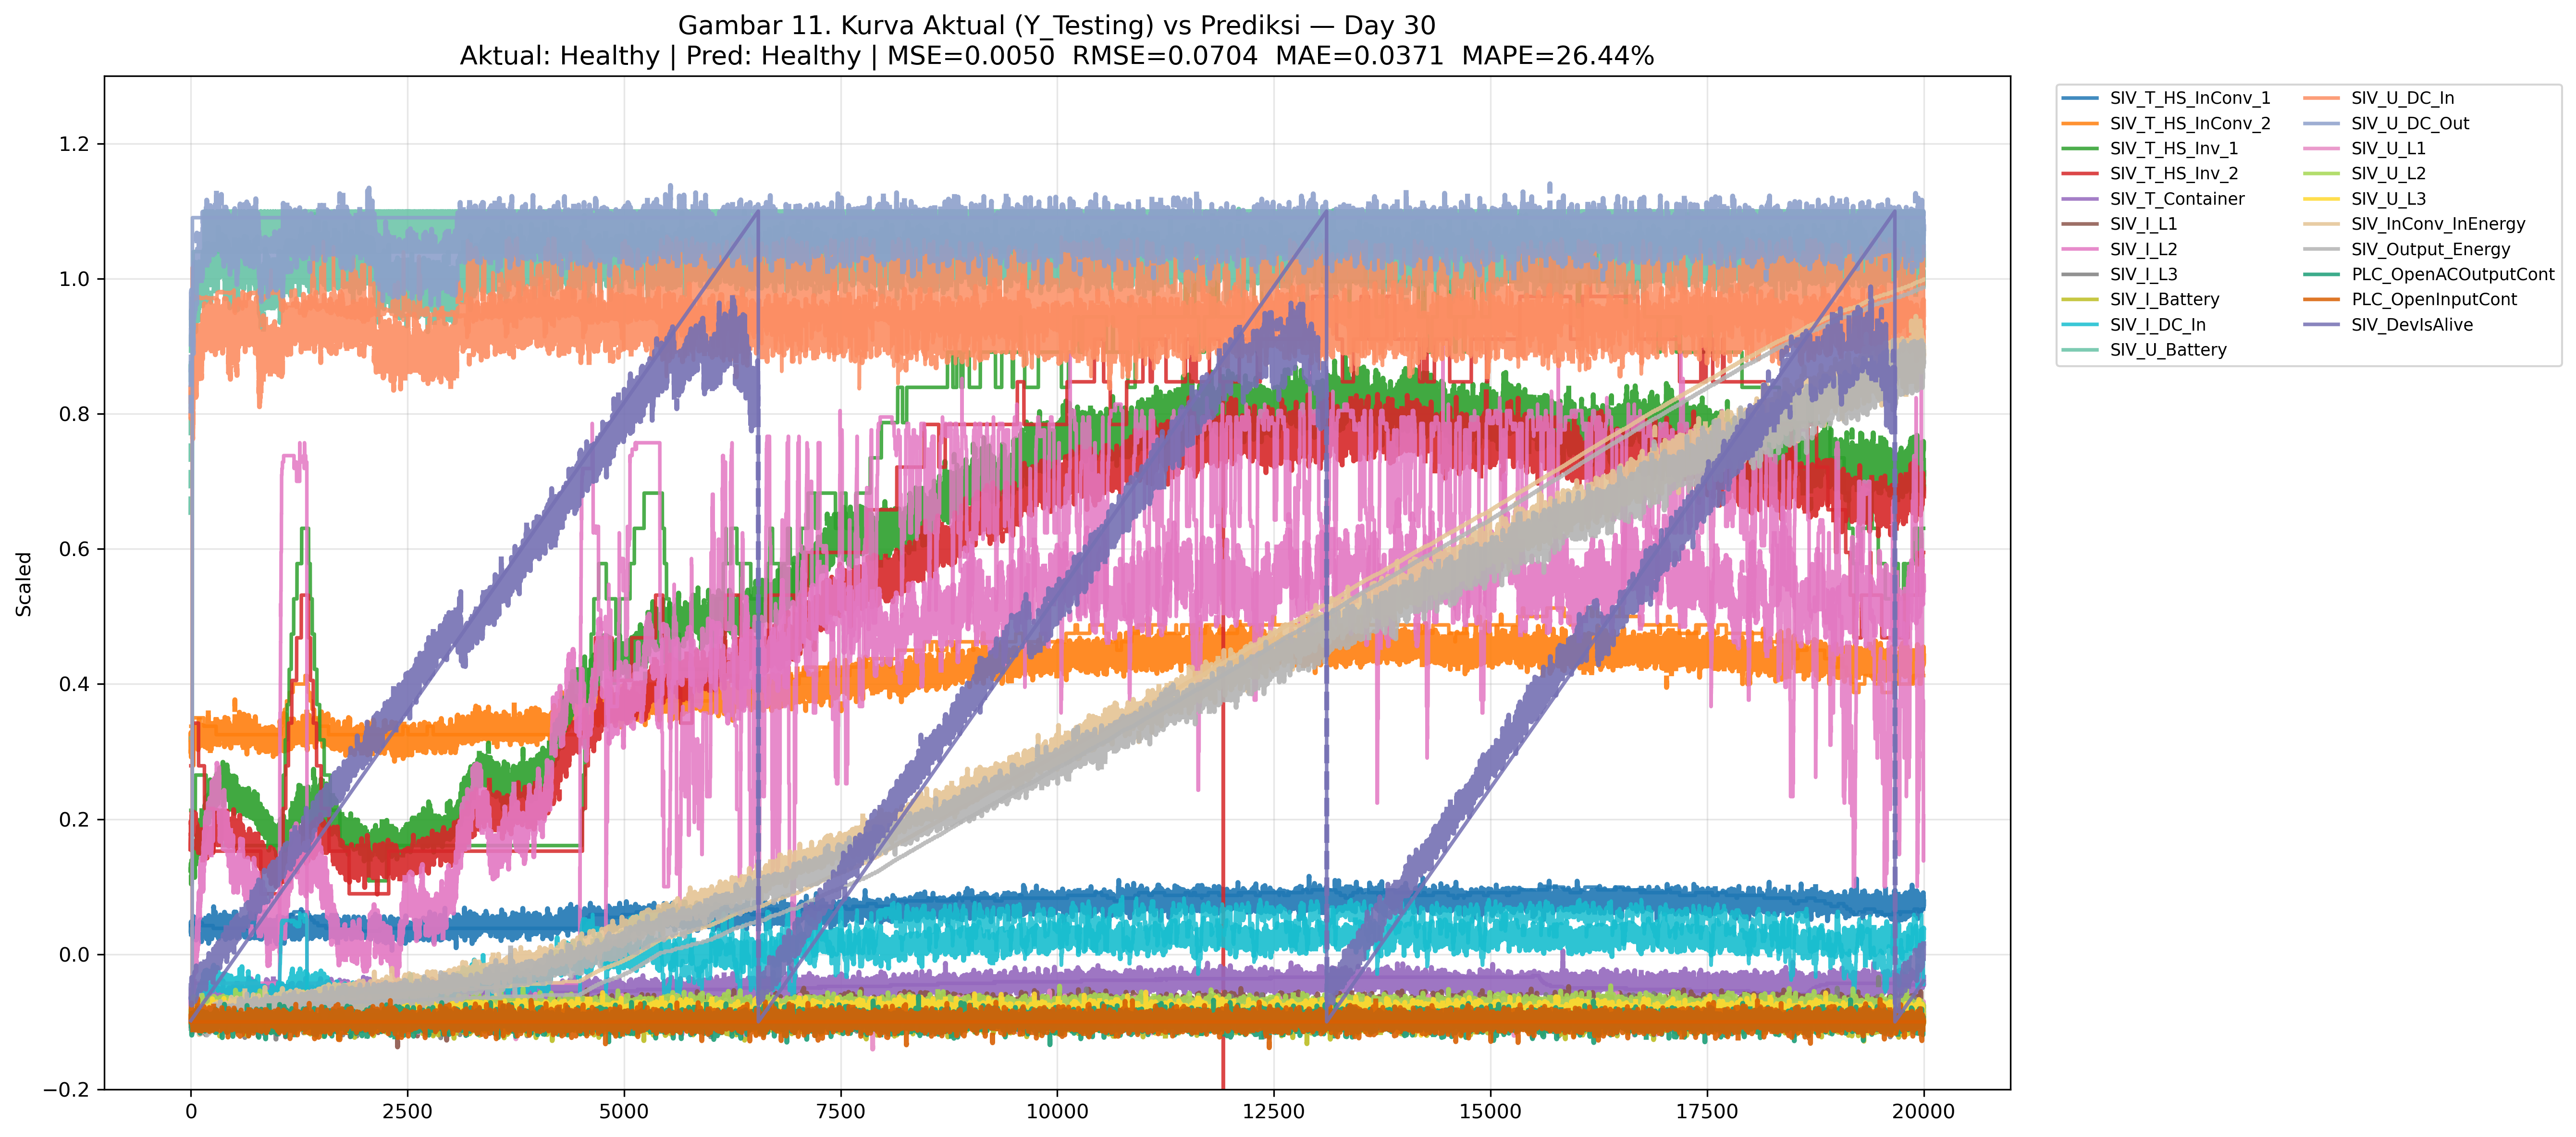
\includegraphics[width=0.85\linewidth]{gambar_train2_real_vs_pred.png}
    \caption{Training Inference — perbandingan aktual vs prediksi.}
    \label{fig:trainrealpred}
\end{figure}

\begin{figure}[H]
    \centering
    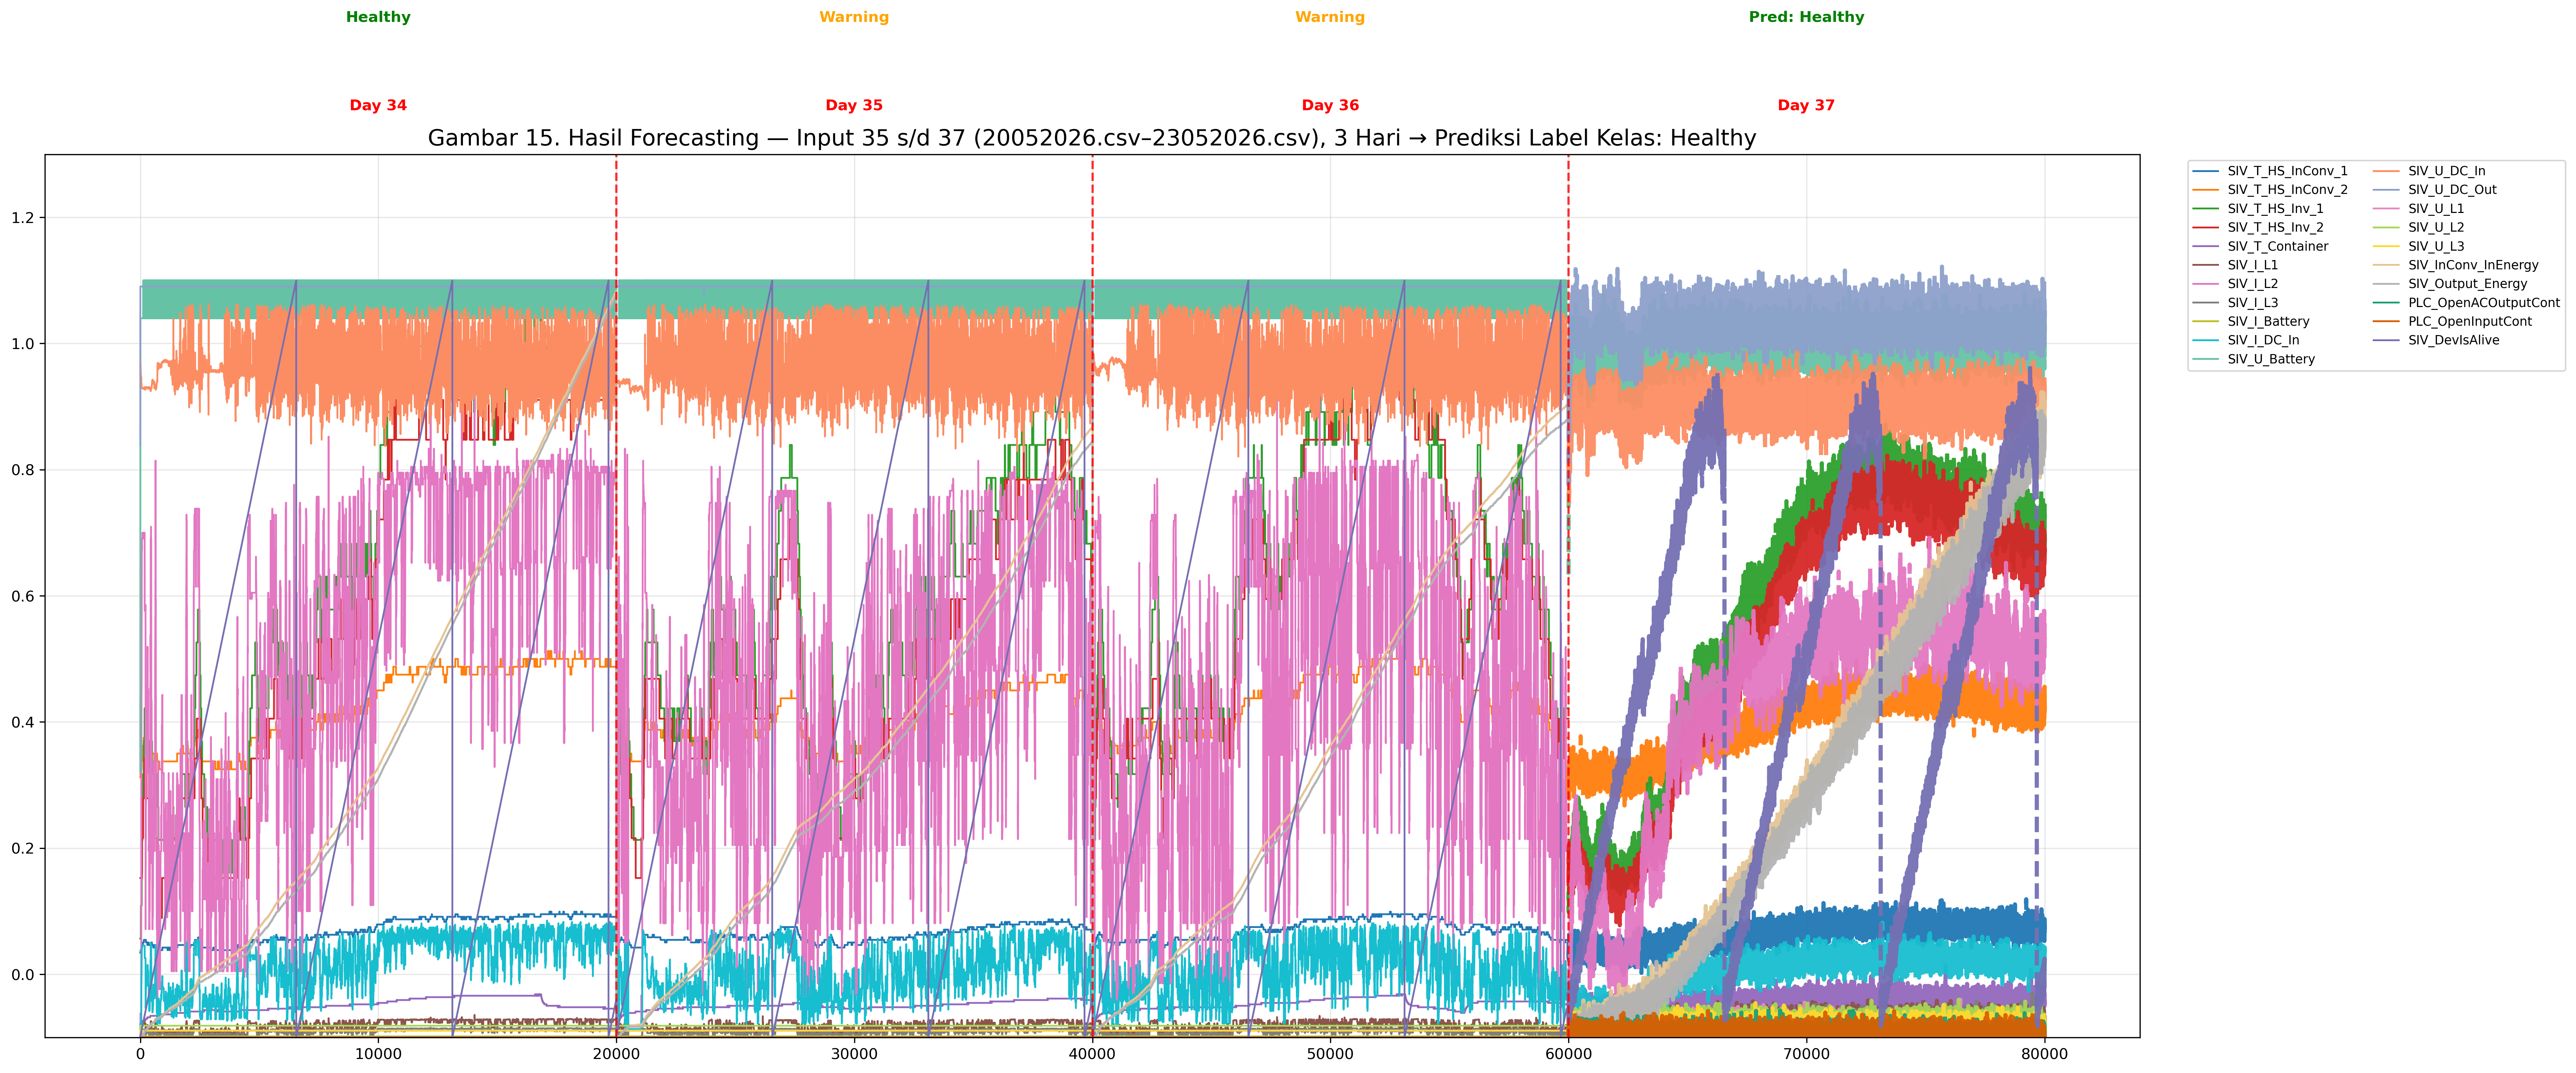
\includegraphics[width=0.85\linewidth]{gambar2_input_plus_prediksi_TCN.png}
    \caption{Testing Inference — hasil forecasting hari ke-38 beserta label kelas prediksi.}
    \label{fig:testforecast}
\end{figure}

% ============================================================
\section{Kesimpulan}
% ============================================================
Model \textbf{TCN Forecaster} berhasil memprediksi 21 parameter sensor SIV TS27 dengan performa baik dan stabil (MSE \textit{test}=0,007446), tanpa indikasi \textit{overfitting}. Model \textbf{MLP Classifier} mencapai akurasi \textit{training} sempurna (100\%) namun turun signifikan pada \textit{testing} (62,5\%, F1=48,08\%), mengindikasikan \textbf{overfitting} akibat keterbatasan data berlabel — terutama kelas \warning\ yang seluruhnya gagal terdeteksi pada data \textit{test}. Tahap \textit{forecasting} terbukti layak digunakan, sedangkan tahap klasifikasi memerlukan penambahan data, \textit{early stopping}, dan regularisasi tambahan sebelum dapat diandalkan sebagai sistem \textit{early warning} operasional. Penelitian lanjutan disarankan mengeksplorasi \textit{k-fold cross-validation}, arsitektur alternatif (LSTM/Transformer), serta pengujian pada unit SIV lain untuk menguji generalisasi lintas unit.

% ============================================================
\section{Lampiran}
% ============================================================
Lampiran berikut memuat rincian data pendukung yang tidak ditampilkan penuh pada badan naskah demi keringkasan, namun disertakan agar seluruh data eksperimen terdokumentasi lengkap.

\subsection{Detail Pembagian Data per Hari}
\begin{longtable}{clcc}
    \toprule
    \textbf{Day} & \textbf{Tanggal} & \textbf{Set} & \textbf{Status Kesehatan} \\
    \midrule
    \endhead
    1  & 02012026 & Train & \warning \\
    2  & 10022026 & Train & \warning \\
    3  & 13022026 & Train & \healthy \\
    4  & 15022026 & Train & \healthy \\
    5  & 19022026 & Train & \healthy \\
    6  & 23022026 & Train & \healthy \\
    7  & 25022026 & Train & \healthy \\
    8  & 01032026 & Train & \warning \\
    9  & 07032026 & Train & \healthy \\
    10 & 22032026 & Train & \warning \\
    11 & 28032026 & Train & \healthy \\
    12 & 08042026 & Train & \healthy \\
    13 & 09042026 & Train & \healthy \\
    14 & 11042026 & Train & \healthy \\
    15 & 12042026 & Train & \healthy \\
    16 & 15042026 & Train & \healthy \\
    17 & 16042026 & Train & \healthy \\
    18 & 17042026 & Train & \healthy \\
    19 & 19042026 & Train & \healthy \\
    20 & 21042026 & Train & \warning \\
    21 & 22042026 & Train & \healthy \\
    22 & 23042026 & Train & \warning \\
    23 & 24042026 & Train & \healthy \\
    24 & 27042026 & Train & \warning \\
    25 & 04052026 & Train & \healthy \\
    26 & 05052026 & Train & \warning \\
    27 & 06052026 & Train & \warning \\
    28 & 07052026 & Train & \healthy \\
    29 & 08052026 & Train & \healthy \\
    30 & 09052026 & Test  & \healthy \\
    31 & 14052026 & Test  & \warning \\
    32 & 15052026 & Test  & \healthy \\
    33 & 16052026 & Test  & \healthy \\
    34 & 17052026 & Test  & \healthy \\
    35 & 20052026 & Test  & \warning \\
    36 & 22052026 & Test  & \warning \\
    37 & 23052026 & Test  & \healthy \\
    \bottomrule
    \caption{Detail 37 hari data beserta pembagian set dan status kesehatan aktual.}
    \label{tab:days}
\end{longtable}

\subsection{Rentang Normalisasi 21 Parameter}
\begin{longtable}{lrr}
    \toprule
    \textbf{Parameter} & \textbf{Min Data} & \textbf{Max Data} \\
    \midrule
    \endhead
    SIV\_T\_HS\_InConv\_1   & 0,0000   & 295,0000 \\
    SIV\_T\_HS\_InConv\_2   & 0,0000   & 96,0000 \\
    SIV\_T\_HS\_Inv\_1      & 31,0000  & 54,0000 \\
    SIV\_T\_HS\_Inv\_2      & 31,0000  & 50,0000 \\
    SIV\_T\_Container       & 30,0000  & 557,0000 \\
    SIV\_I\_L1              & 0,0000   & 4144,0000 \\
    SIV\_I\_L2              & 0,0000   & 126,0000 \\
    SIV\_I\_L3              & 0,0000   & 8198,0000 \\
    SIV\_I\_Battery         & -33,0000 & 24800,0000 \\
    SIV\_I\_DC\_In          & 0,0000   & 544,0000 \\
    SIV\_U\_Battery         & 94,0000  & 114,0000 \\
    SIV\_U\_DC\_In          & 0,0000   & 936,0000 \\
    SIV\_U\_DC\_Out         & 3,0000   & 127,0000 \\
    SIV\_U\_L1              & 0,0000   & 24768,0000 \\
    SIV\_U\_L2              & 0,0000   & 14272,0000 \\
    SIV\_U\_L3              & 0,0000   & 24603,0000 \\
    SIV\_InConv\_InEnergy   & 0,0000   & 644,0000 \\
    SIV\_Output\_Energy     & 0,0000   & 574,0000 \\
    PLC\_OpenACOutputCont   & 0,0000   & 0,0000 \\
    PLC\_OpenInputCont      & 0,0000   & 0,0000 \\
    SIV\_DevIsAlive         & 0,0000   & 65535,0000 \\
    \bottomrule
    \caption{Rentang nilai (min--max) 21 parameter dari scaler training.}
    \label{tab:minmax}
\end{longtable}

\subsection{Pembentukan Sequence Sliding Window}
\begin{longtable}{clllll}
    \toprule
    \textbf{Seq} & \textbf{Input A} & \textbf{Input B} & \textbf{Input C} & \textbf{Target H+1} & \textbf{Set} \\
    \midrule
    \endhead
    1  & 02012026 & 10022026 & 13022026 & 15022026 & Training \\
    2  & 10022026 & 13022026 & 15022026 & 19022026 & Training \\
    3  & 13022026 & 15022026 & 19022026 & 23022026 & Training \\
    4  & 15022026 & 19022026 & 23022026 & 25022026 & Training \\
    5  & 19022026 & 23022026 & 25022026 & 01032026 & Training \\
    6  & 23022026 & 25022026 & 01032026 & 07032026 & Training \\
    7  & 25022026 & 01032026 & 07032026 & 22032026 & Training \\
    8  & 01032026 & 07032026 & 22032026 & 28032026 & Training \\
    9  & 07032026 & 22032026 & 28032026 & 08042026 & Training \\
    10 & 22032026 & 28032026 & 08042026 & 09042026 & Training \\
    11 & 28032026 & 08042026 & 09042026 & 11042026 & Training \\
    12 & 08042026 & 09042026 & 11042026 & 12042026 & Training \\
    13 & 09042026 & 11042026 & 12042026 & 15042026 & Training \\
    14 & 11042026 & 12042026 & 15042026 & 16042026 & Training \\
    15 & 12042026 & 15042026 & 16042026 & 17042026 & Training \\
    16 & 15042026 & 16042026 & 17042026 & 19042026 & Training \\
    17 & 16042026 & 17042026 & 19042026 & 21042026 & Training \\
    18 & 17042026 & 19042026 & 21042026 & 22042026 & Training \\
    19 & 19042026 & 21042026 & 22042026 & 23042026 & Training \\
    20 & 21042026 & 22042026 & 23042026 & 24042026 & Training \\
    21 & 22042026 & 23042026 & 24042026 & 27042026 & Training \\
    22 & 23042026 & 24042026 & 27042026 & 04052026 & Training \\
    23 & 24042026 & 27042026 & 04052026 & 05052026 & Training \\
    24 & 27042026 & 04052026 & 05052026 & 06052026 & Training \\
    25 & 04052026 & 05052026 & 06052026 & 07052026 & Training \\
    26 & 05052026 & 06052026 & 07052026 & 08052026 & Training \\
    27 & 06052026 & 07052026 & 08052026 & 09052026 & Testing \\
    28 & 07052026 & 08052026 & 09052026 & 14052026 & Testing \\
    29 & 08052026 & 09052026 & 14052026 & 15052026 & Testing \\
    30 & 09052026 & 14052026 & 15052026 & 16052026 & Testing \\
    31 & 14052026 & 15052026 & 16052026 & 17052026 & Testing \\
    32 & 15052026 & 16052026 & 17052026 & 20052026 & Testing \\
    33 & 16052026 & 17052026 & 20052026 & 22052026 & Testing \\
    34 & 17052026 & 20052026 & 22052026 & 23052026 & Testing \\
    \bottomrule
    \caption{Detail pembentukan 34 sequence sliding-window (3 hari input $\to$ 1 hari target).}
    \label{tab:seq}
\end{longtable}

\subsection{Gambar Pendukung Tambahan}
\begin{figure}[H]
    \centering
    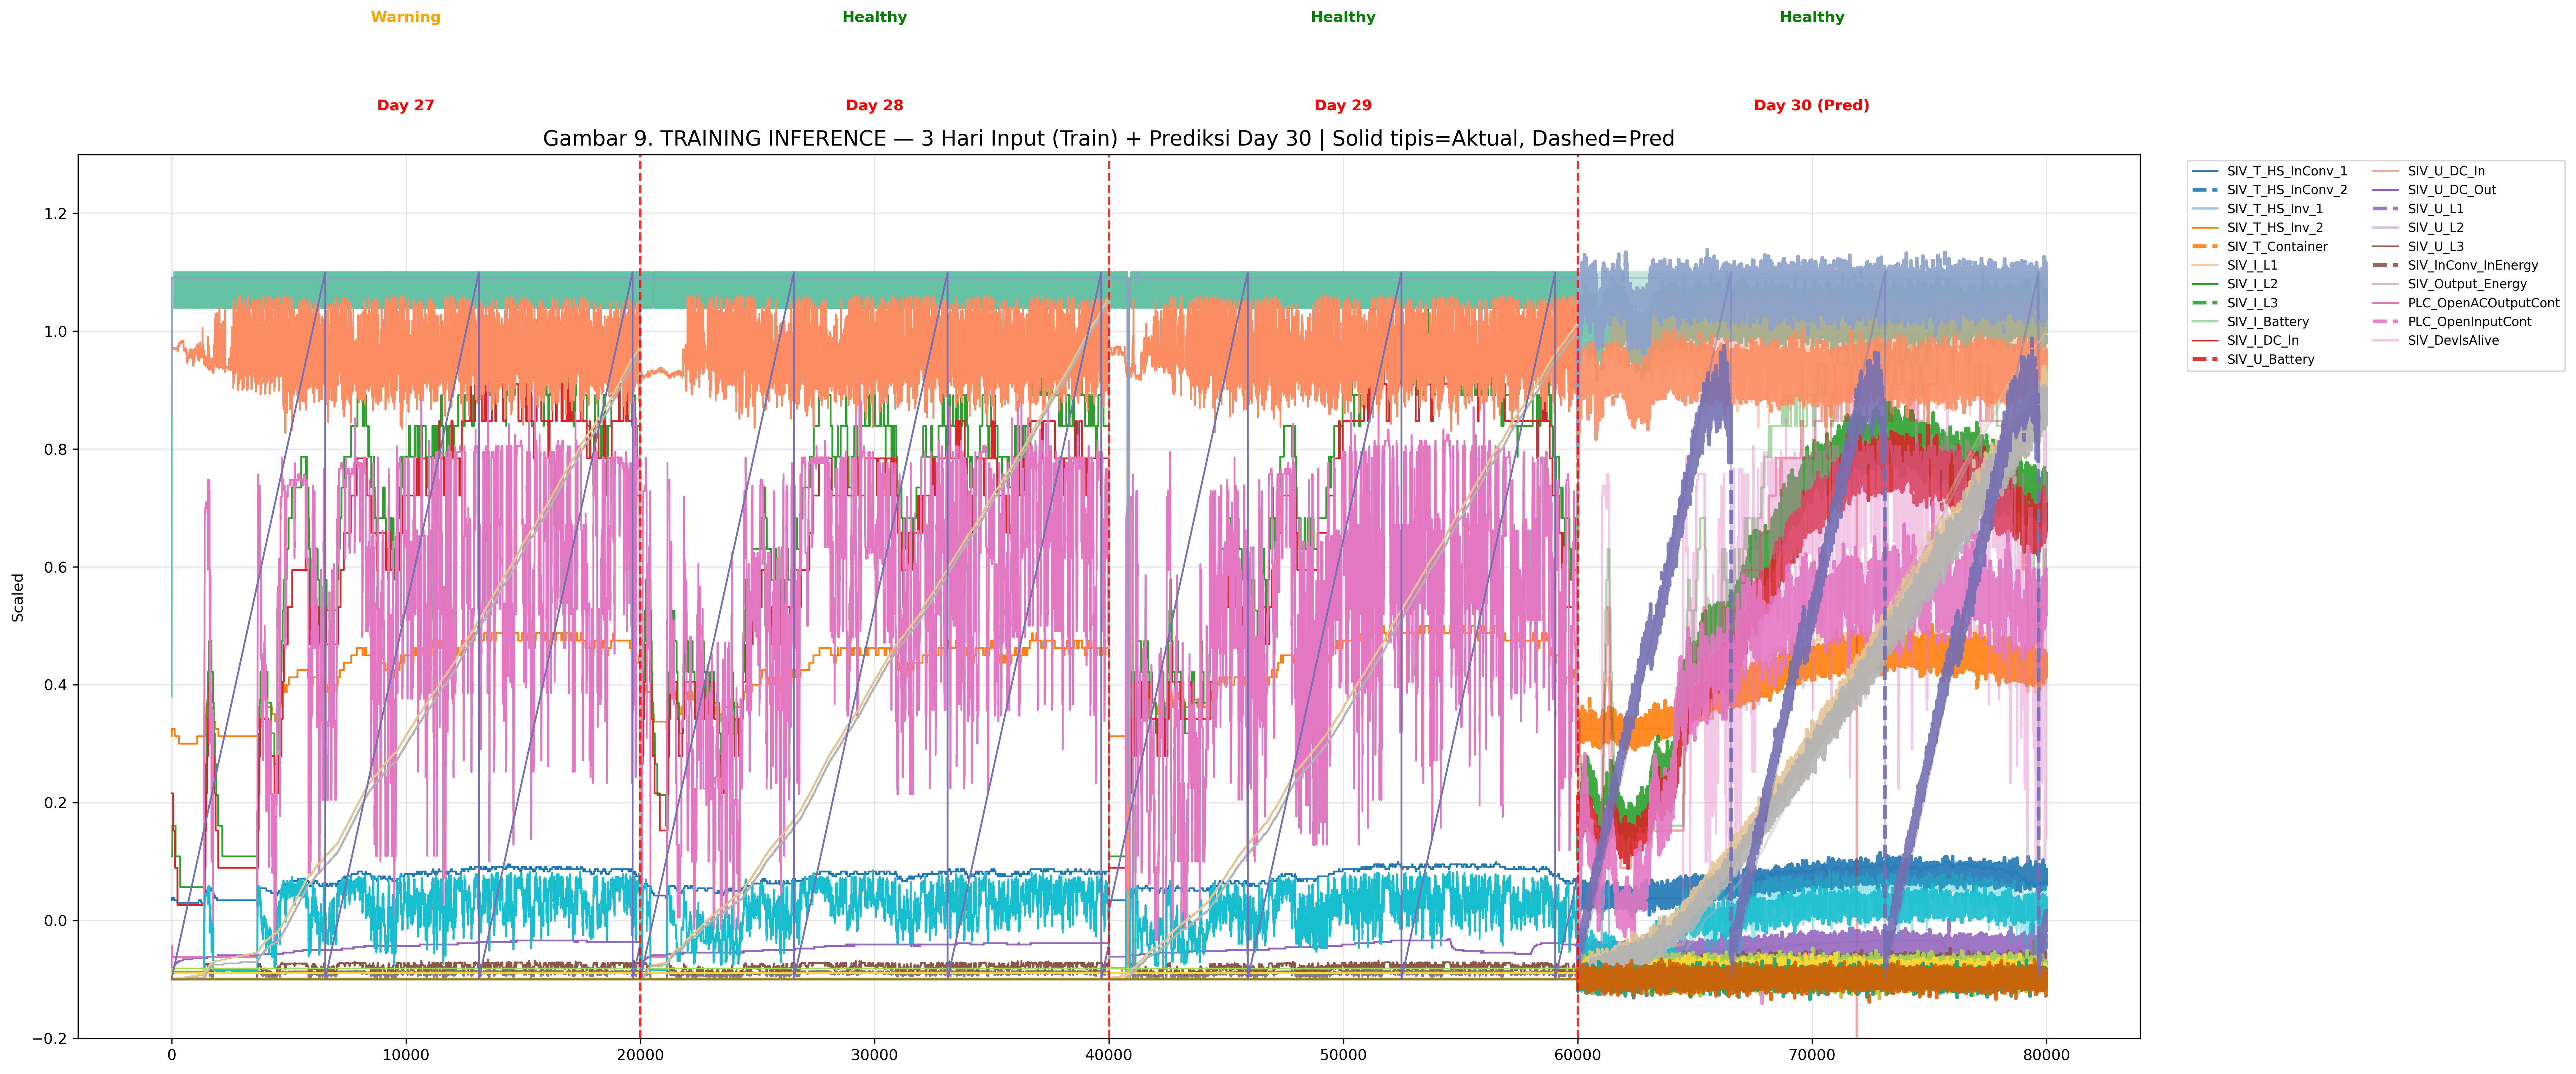
\includegraphics[width=0.8\linewidth]{gambar_train1_input_prediksi.png}
    \caption{Training Inference — 3 hari input training + hasil prediksi.}
    \label{fig:traininput}
\end{figure}

\begin{figure}[H]
    \centering
    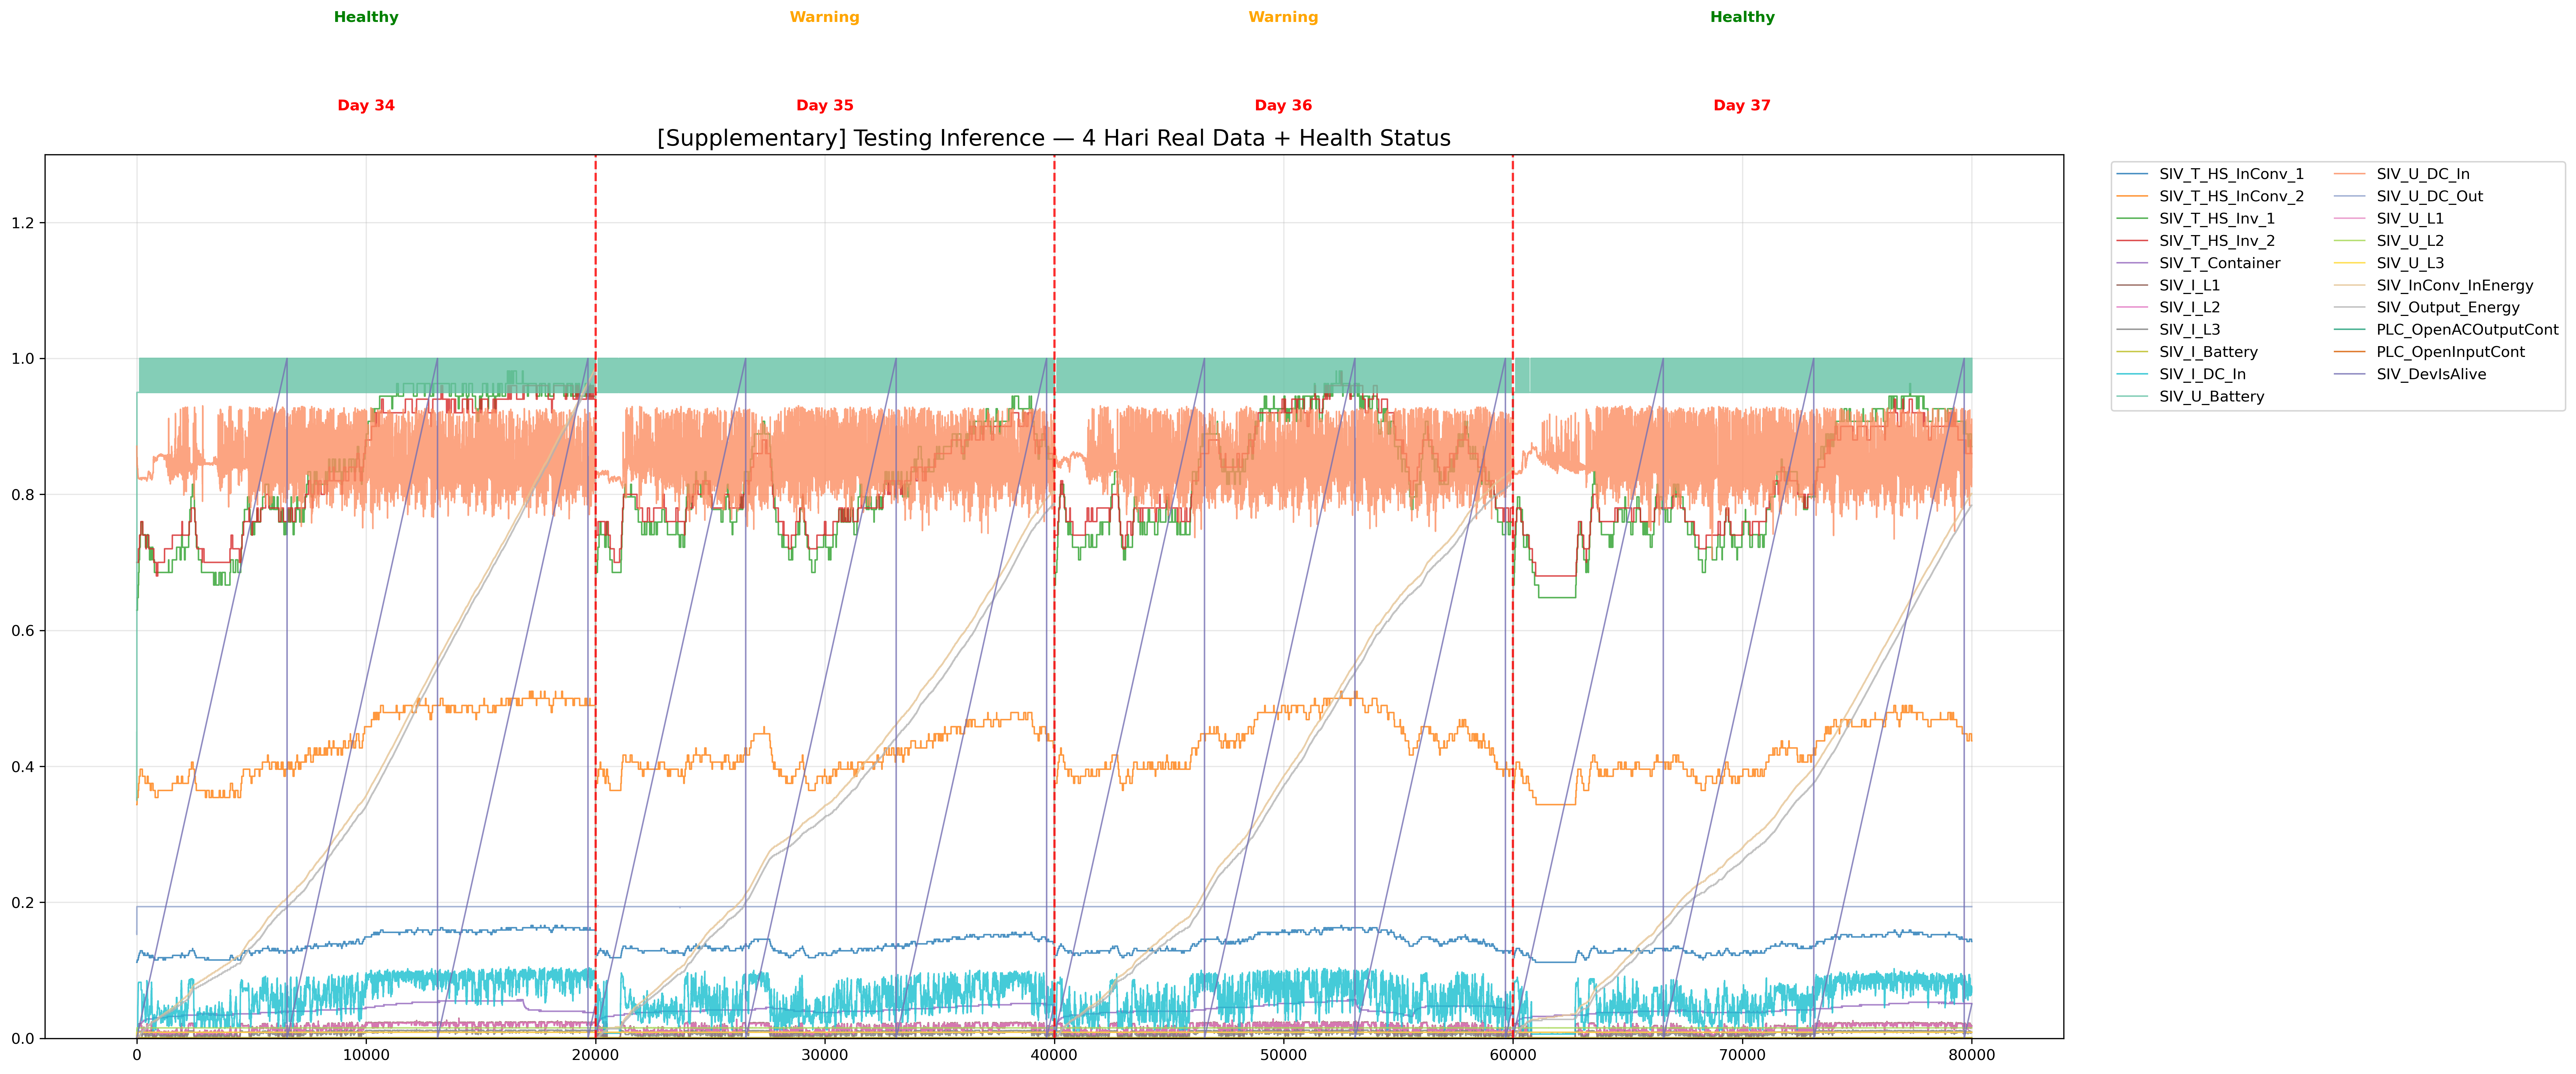
\includegraphics[width=0.8\linewidth]{gambar1_4hari_real_TCN.png}
    \caption{Konteks 4 hari data real menjelang Testing Inference.}
    \label{fig:4hari}
\end{figure}

\begin{figure}[H]
    \centering
    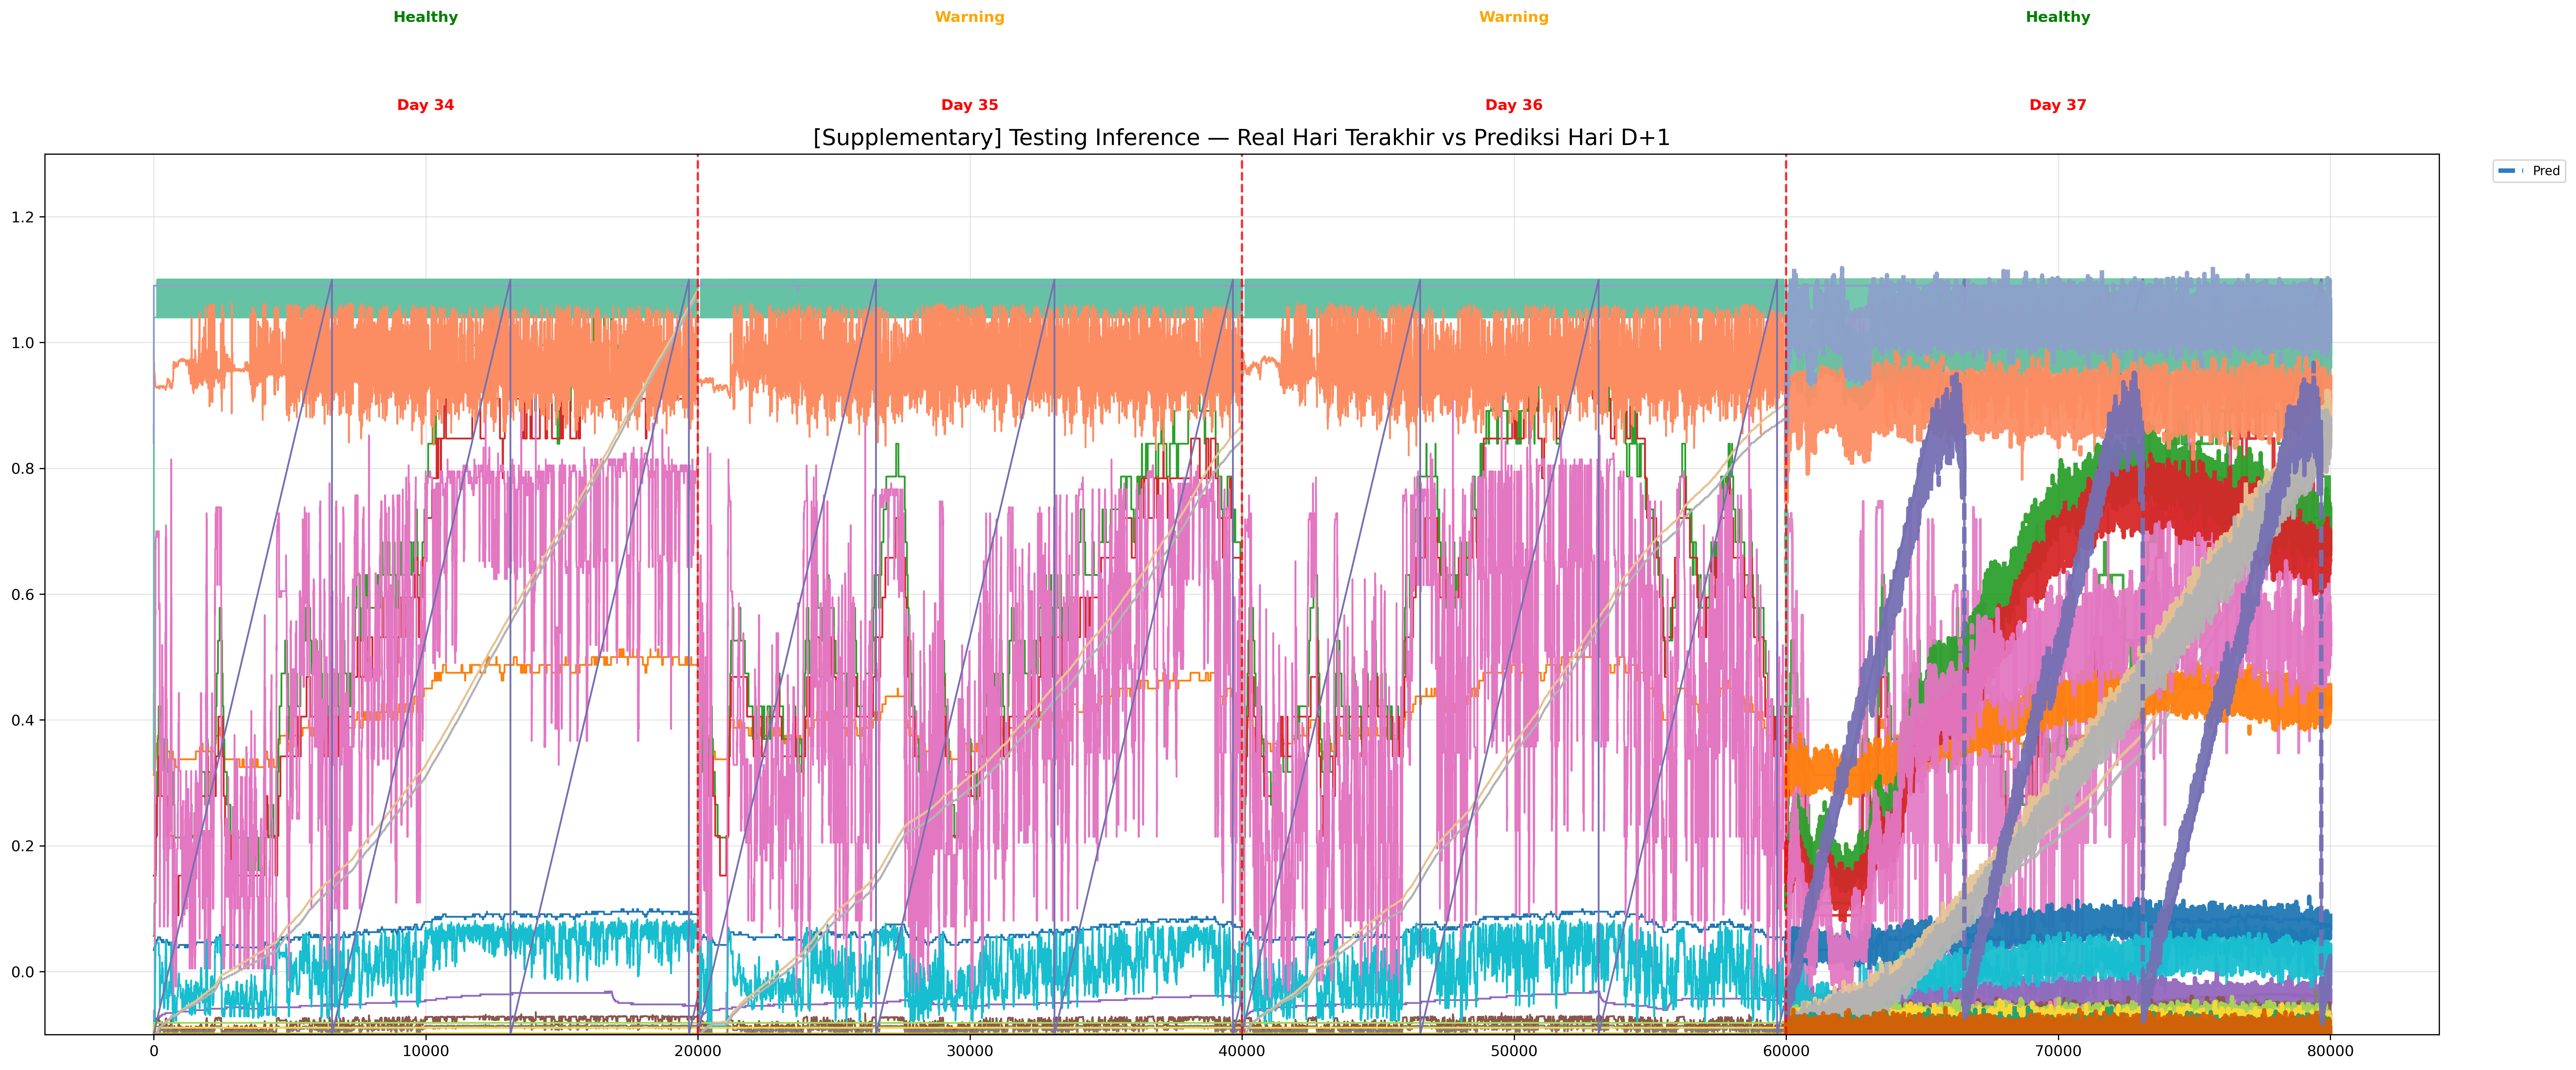
\includegraphics[width=0.8\linewidth]{gambar3_real_vs_prediksi_TCN.png}
    \caption{Overlay data real vs prediksi pada Testing Inference.}
    \label{fig:testrealpred}
\end{figure}

\subsection{Daftar File Output}
\begin{table}[H]
    \centering
    \small
    \caption{Daftar file data dan model pendukung.}
    \begin{tabular}{ll}
        \toprule
        \textbf{Nama File} & \textbf{Deskripsi} \\
        \midrule
        jurnal\_info\_stage1.txt & Hyperparameter, MSE train/test, tabel sequence \\
        jurnal\_info\_stage2.txt & Hyperparameter, CE/Acc, confusion matrix \\
        jurnal\_fitur\_statistik.csv & Mean/std/max/min per parameter per hari (84 kolom) \\
        inference\_train\_health\_status.csv & Hasil training inference \\
        inference\_health\_status.csv & Hasil testing inference \\
        model\_stage1\_forecaster.pth & Bobot model TCN terlatih \\
        model\_stage2\_classifier.pth & Bobot model MLP terlatih \\
        log\_stage1.txt / log\_stage2.txt & Log lengkap proses training \\
        \bottomrule
    \end{tabular}
\end{table}

% ============================================================
\section*{Daftar Pustaka}
% ============================================================
\textit{[Lengkapi daftar pustaka sesuai gaya sitasi jurnal tujuan (APA/IEEE). Contoh format IEEE:]}
\begin{enumerate}[label={[\arabic*]}]
    \item [Nama Penulis], "[Judul artikel]," \textit{[Nama Jurnal/Konferensi]}, vol. [x], no. [x], pp. [xx-xx], [Tahun].
    \item [Nama Penulis], \textit{[Judul Buku]}. [Kota]: [Penerbit], [Tahun].
\end{enumerate}

\end{document}
